% Document
\documentclass[12pt, a4paper]{article}
\usepackage[T1]{fontenc}
\usepackage[utf8]{inputenc}
\usepackage{authblk}
\usepackage{lipsum}
\usepackage{hyperref}

% Figure and table formating
\usepackage{epsfig}
\usepackage{tabu}
\usepackage{rotating}
\usepackage{pbox}
\usepackage{framed, multicol}
\usepackage[framemethod=TikZ]{mdframed}
\usepackage{float}
\usepackage[left=1.25 in, right=1.25 in, top=1.25 in, bottom=1.25 in]{geometry}

% Fonts - Mathtime
%\usepackage{txfonts}
\usepackage{amsmath} % Add amssymb if not using Mathtime

% Text
\setlength{\parindent}{0.5in}
\frenchspacing  \tolerance = 800  \hyphenpenalty = 800

\usepackage{lineno} % Line numbers
\def\linenumberfont{\normalfont\footnotesize\ttfamily}
\setlength\linenumbersep{0.2 in}

\usepackage{setspace}

% Format section and subsection headers
\makeatletter
\renewcommand{\section}{\@startsection
{section}%                   % the name
{1}%                         % the level
{0mm}%                       % the indent
{-\baselineskip}%            % the before skip
{0.5\baselineskip}%          % the after skip
{\normalfont\bf\large}} % the style

\renewcommand{\subsection}{\@startsection
{subsection}%                   % the name
{2}%                         % the level
{0mm}%                       % the indent
{-\baselineskip}%            % the before skip
{0.5\baselineskip}%          % the after skip
{\normalfont\bf}} % the style
\makeatother

% Other
\usepackage{graphicx}
\usepackage[singlelinecheck=false,font=small,labelfont=bf]{caption}

% Bibliography
\usepackage[numbers, compress]{natbib} % Bibliography - APA
\bibpunct{(}{)}{;}{a}{}{,}

% Format the Bibliography appropriately
% increase \bibhang to take care of the numbers
\setlength{\bibhang}{0pc}
\makeatletter
% patch \@lbibitem to print the current number before the authors
\patchcmd{\@lbibitem}
  {]}
  {] \theNAT@ctr. \newline }
  {}{}
\makeatother


%%%%%% FRONT MATTER %%%%%%%%%

\begin{document}

\linenumbers

\doublespacing

\noindent
\Large{\textbf{Supporting Information}}

\normalsize

\section*{SI 1: Implementation of the Crofton Method}

The algorithm for fitting the Crofton Method \citep{Crofton1971a} proceeds as follows. First, obtain a dataset
with $n$ hosts where each host has some parasite intensity 0 to $p_{max}$. Starting
with the full dataset, guess a vector of pre-mortality parameters $(N_{p1}, \mu_{p1}, k_{p1})$ where $N_{p1}$ is the total number of hosts before mortality, $\mu_{p1}$ is the parasite intensity before mortality, and $k_{p1}$ is the parasite aggregation before mortality. Given
these parameters, use a negative binomial distribution to calculate the predicted number of hosts with $0, 1, 2, \dots
p_{max}$ parasites.  Compare the expected number of hosts with $0, 1, 2, \dots  p_{max}$ parasites
to the observed number hosts with $0, 1, 2, \dots p_{max}$ parasites and calculate
the $\chi^2$-squared statistic associated with the observed and predicted vectors. In reality, one often has to bin the parasite intensity data because all
parasite intensities are not represented in the dataset. Continue to guess $(N_{p1},
\mu_{p1}, k_{p1})$ vectors until a set of parameters is found that minimizes the $\chi^2$-
squared statistic.

Second, choose a truncation value ($t_2$) such that $t_2 <
p_{max}$. Truncate the data such that $\text{data}_\text{truncated} <= t_2$ and repeat the above
iterative procedure to calculate another set of parameters $(N_{p2}, \mu_{p2}, k_{p2})$
that minimizes the $\chi^2$-squared statistic on the truncated data. Choose a new
truncated value $t_3 < t_2$ and repeat the first two steps. Continue to truncate
the dataset until it only contains hosts with 0, 1, and 2 parasites (or 3 bins).
Because the method attempts to estimate three parameters, at least 3 classes are
needed for all 3 parameters to be identifiable \citep{Royce1990}.


Once the iterative procedure has been completed, parasite-induced host mortality is traditionally identified by plotting the different truncation values $t_{i}$ against the different values of $N_{pi}$ and looking for a distinct ``kink'' in the resulting plot.   Once the ``kink'' as occurred, the values of $N_{pi}$ will typically remain close to constant as $t_i$ is decreased further.  The ``true'' pre-mortality parameters $N_{pt}$, $\mu_{pt}$, and $k_{pt}$ are taken to be at the point where the ``kink'' occurs.

We provide an implementation and unit tests of the Crofton Method in  Supplementary Information 4.  Figure \ref{fig:crof_test} visually shows that our implementation of the Crofton Method agrees with results previously published by \cite{Crofton1971a}.

\section*{SI 2: Implementation of the Adjei Method}

The Adjei Method for estimating PIHM has two steps \citep{Adjei1986}.  The first
step is to estimate the parameters of the pre-mortality host-parasite
distribution using the Crofton Method (see \emph{SI} 1).  The three parameters estimated are the
total number of hosts before mortality $N_p$,  the mean number of parasites per
host before mortality $\mu_p$, and the aggregation of parasites before
mortality given by the parameter $k_p$ from a negative binomial distribution.
When $k_p$ is small, parasites are highly aggregated among hosts and when
$k_p$ is large parasites are more evenly distributed across hosts \citep{Wilson2002}.  The implementation of the Crofton Method has been discussed at length elsewhere \citep[e.g.][ and in \emph{SI} 1]{Royce1990,Lester1984} and we provide a tested implementation of the method in \emph{SI} 4.

The second step of the Adjei Method is to make the assumption that infection, host mortality, and sampling occur in that order and are temporally \cite{Adjei1986}. Next, \citeauthor{Adjei1986} assume that the host survival function follows the logistic form

\begin{equation}
    h(\text{survival}; x, a, b) = \dfrac{\exp{(a - b \log(x))}}{1 + \exp{(a - b \log(x))}}
    \label{eq:logistic}
\end{equation}
where $x$ is the parasite intensity in a given host and $a$ and $b$ are the two
parameters of the logistic function. Generally, a larger $a$ allows for hosts to
tolerate larger parasite intensities before experiencing parasite-induced mortality
and a larger $b$ leads to a more rapid decline in the probability of host
survival as parasite intensity increases. The value $\exp(a / b)$ is referred
to as the $LD_{50}$. Individuals with loads higher than this will have a greater than 50\% chance of death.

By taking the first and second derivatives of equation \ref{eq:logistic}, one can easily find that the maximum rate of decline in host survival probability with increasing parasite intensity occurs at the $LD_{50}$ and has a value of $b / 4$.  This is in many ways analogous to the parasite pathogenicity parameter $\alpha$ given in classic macroparasite models, which specifies the slope of the linear relationship between between host death rate and parasite intensity \citep{AndersonandMay1978, Isham1995}.  The parameter $a$ is easily interpreted by holding $b$ constant and looking at how a one unit change in $a$ affects the log parasite intensity at which some percentage $p$ of hosts experience mortality.  Letting $a_1$ and $a_2$ be two different values of $a$ and $x_1$ and $x_2$ be two different parasite intensities, a bit of rearranging of equation \ref{eq:logistic} gives.

\begin{align*}
    \log{\frac{p}{1 - p}} &= a_1 - b \log{x_1}\\
    - \log{\frac{p}{1 - p}} &= a_1 - b \log{x_2}\\
    0 &= a_1 - a_2 - b\log{x_1} + b\log{x_2}\\
    a_2 - a_1 &= b(\log{x_2} - \log{x_1})
\end{align*}
If $a_2 - a_1 = 1$, than the change in log parasite intensity at which $p$ percentage of hosts survive is $1 / b$.

To estimate the parameters in equation \ref{eq:logistic}, the Adjei Method first
calculates the expected number of hosts with a given parasite load $x$ by using
the equation $g(x ; \mu_p, k_p) * N_p$, where $g(x ; \mu_p, k_p)$ is the negative binomial pre-mortality distribution.  Second, the observed and predicted number of hosts
with $x$ parasites are paired as a single data point and the method then assumes that
this data point follows a binomial distribution with the total number of
``trials'' equal to the predicted number of hosts and the total number of
``successes'' equal to the observed number of hosts. In some cases, the
observed number of hosts is greater than the expected number of hosts and the
Adjei Method alters the data so that the observed is equal to the predicted
\citep{Adjei1986}.  After this questionable manipulation, the (observed, predicted) pairs are fit to a standard Generalized Linear Model \citep{McCullagh1989} with a binomial response variable and a logistic link function given by equation \ref{eq:logistic}.  This model provides estimates for parameters $a$, $b$ and $LD_{50}$.

While not included in the original implementation of the Adjei Method, a
$\chi^2$ test with a degrees of freedom of 1 can be used to assess whether a GLM model that includes parasite
intensity as a predictor of host survival probability is a ``better'' model than a
GLM without this predictor.  This allows the Adjei Method to determine whether
PIHM is a significant factor in a host-parasite system.

The Adjei Method's most glaring deficiency is the need to alter the observed
data in order to fit the model into the binomial GLM framework.  A second more
subtle problem with the Adjei Method is the potential need to bin data in order
to predict greater than one host in a given parasite intensity class.  For
example, if the total number of hosts pre-mortality was 50, the mean number of
parasites per host pre-mortality was 100 and the aggregation parameter was 1, applying the equation $g(x ; \mu_p=100, k_p=1) * 50$ would result in
less than 1 individual in all parasite intensities $x$. In other words, the
Adjei Method cannot be applied to samples with either very high mean parasite
loads, small sample sizes, or both without some sort of binning of the data.
While this is not a flaw \emph{per se}, it does add a certain level of
subjectivity (i.e. which bins should you use?) to a method that already has
serious potential issues.  In this analysis, we always assume the Adjei Method is not binning the data, though we provide code for applying the binning method in SI 4.


\section*{SI 3: Additional Figures}

See Figures 1 - 9.

\section*{SI 4: Code and unit tests for estimating parasite-induced host mortality}

Python code, unit tests, and a help file for the Crofton Method, the Adjei Method and the Likelihood Method can be found at \url{https://github.com/mqwilber/parasite_mortality}


\singlespacing
\bibliographystyle{int_j_para.bst}
\bibliography{parasite_host_mortality}

\begin{figure}

    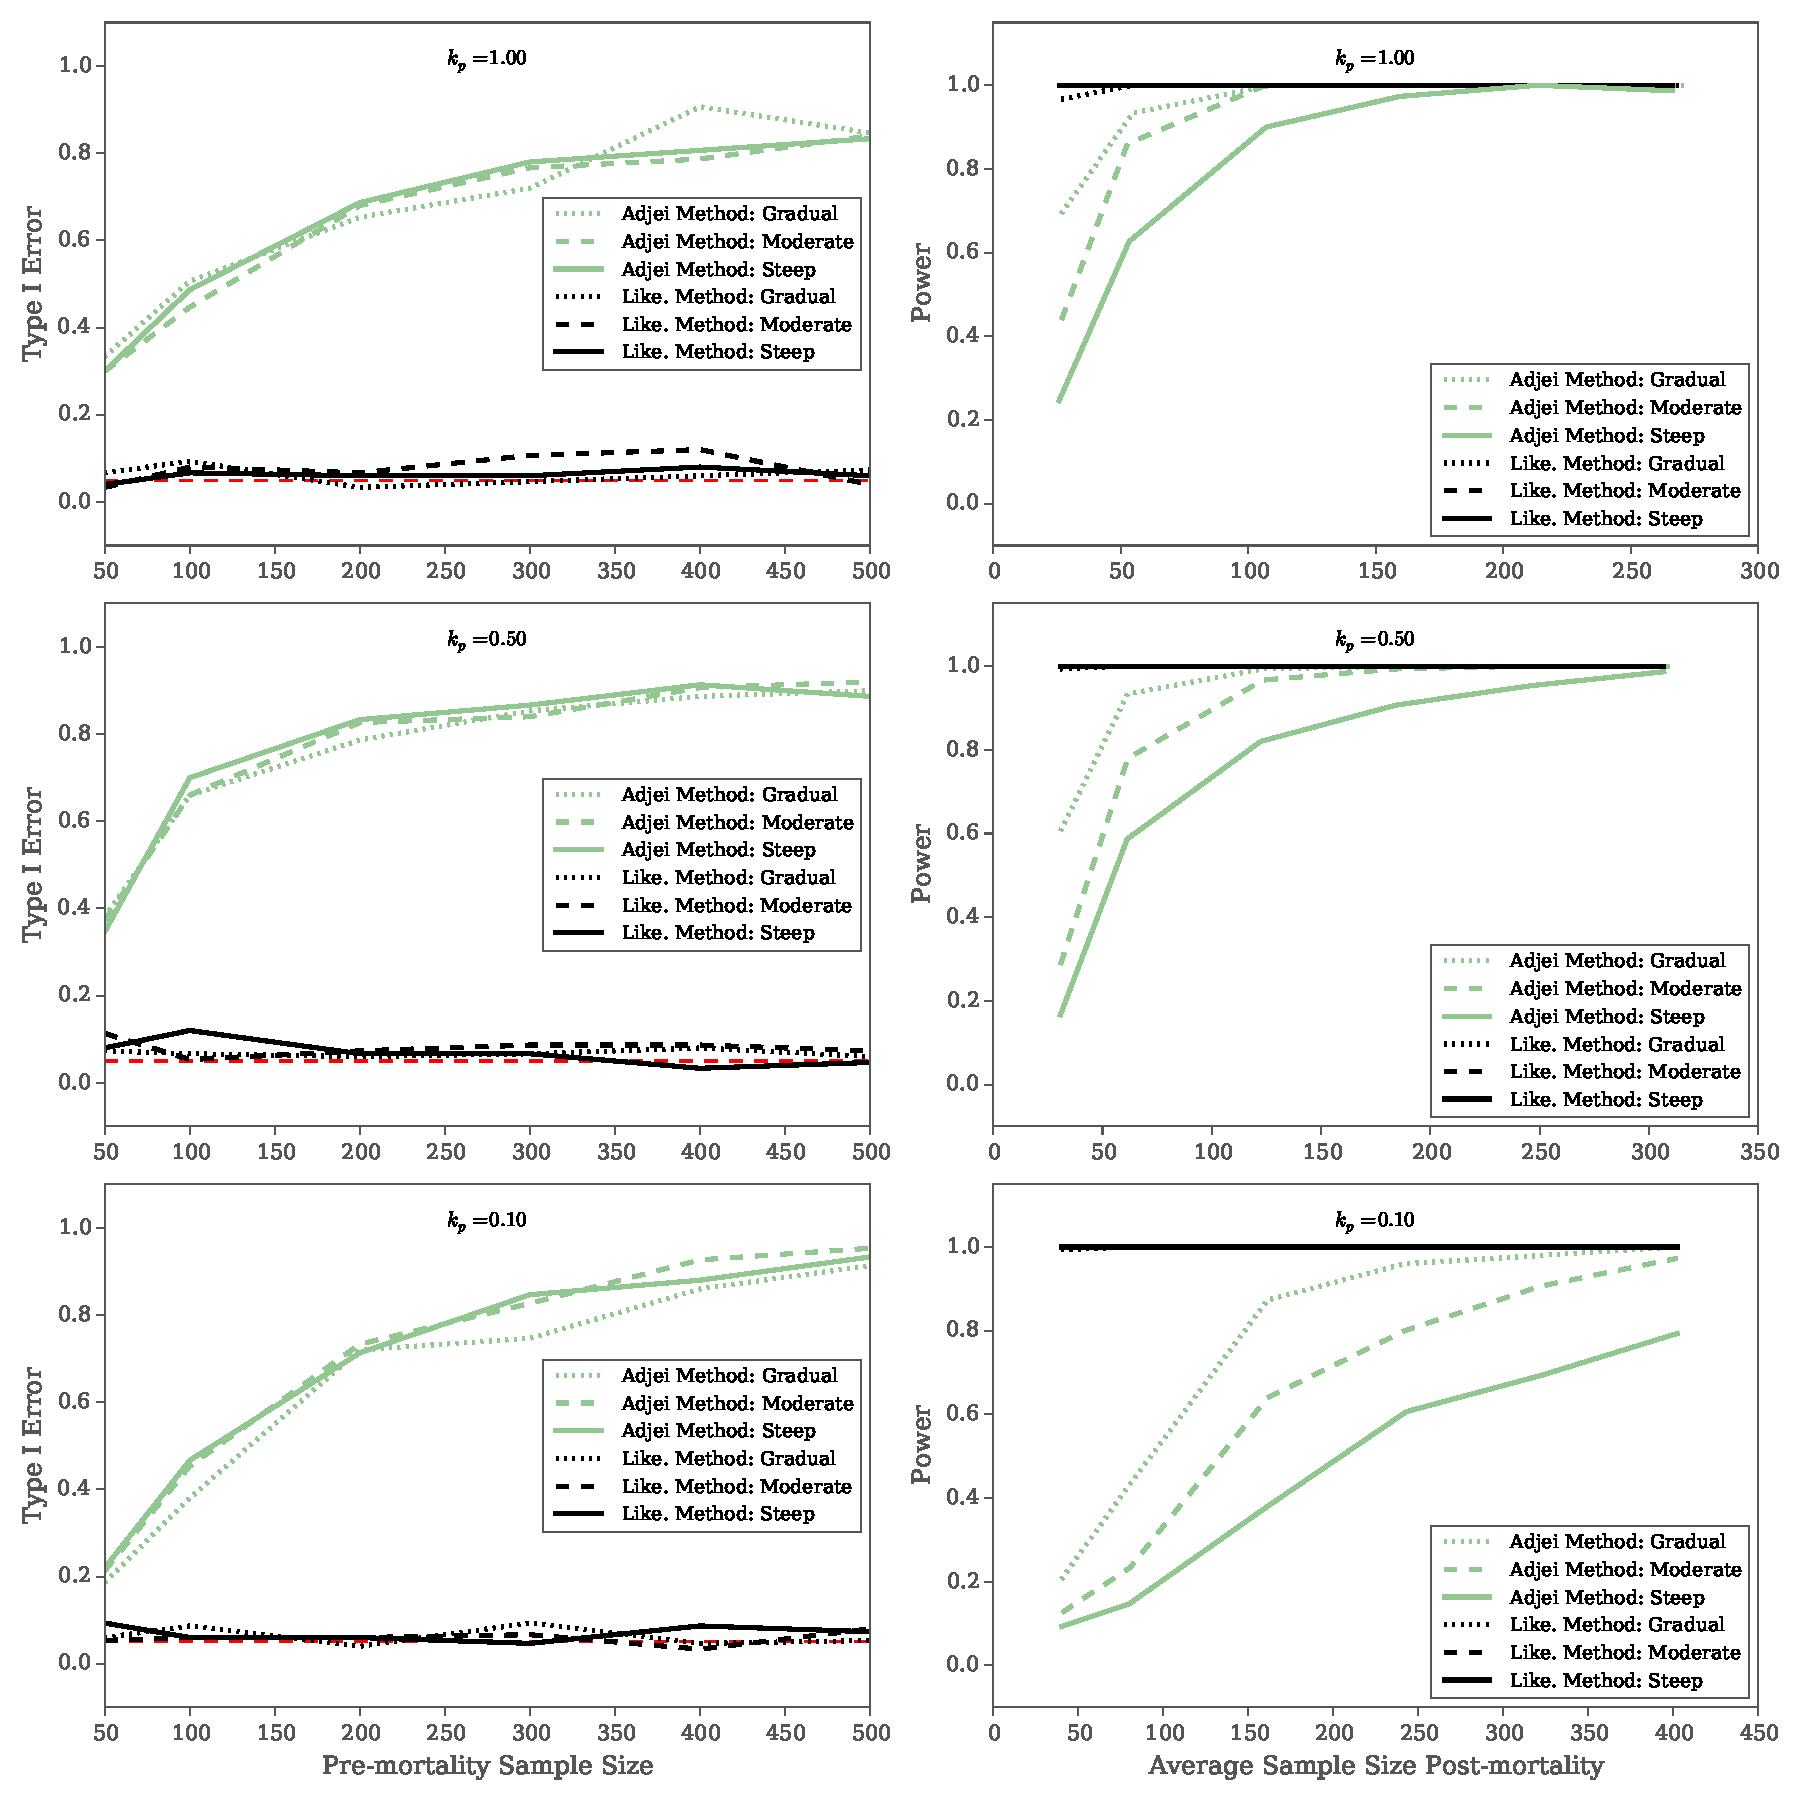
\includegraphics[width=\textwidth]{/Users/mqwilber/Repos/parasite_mortality/results/typeIpower_figure_for_mu10}

    \caption{The type I error rate and the power of the Likelihood Method (solid line) and the Adjei Method (dashed lines) when $\mu_p = 10$ for various shapes of the host survival function and levels of aggregation $k_p$.  The first column gives the type I error rate of each method for falsely detecting PIHM when none is present.  The red line gives the the pre-set type I error rate of $\alpha = 0.05$.  The second column gives the power of a given method to detect PIHM when it is actually occurring. }
    \label{fig:typeI10}

\end{figure}

\begin{figure}

    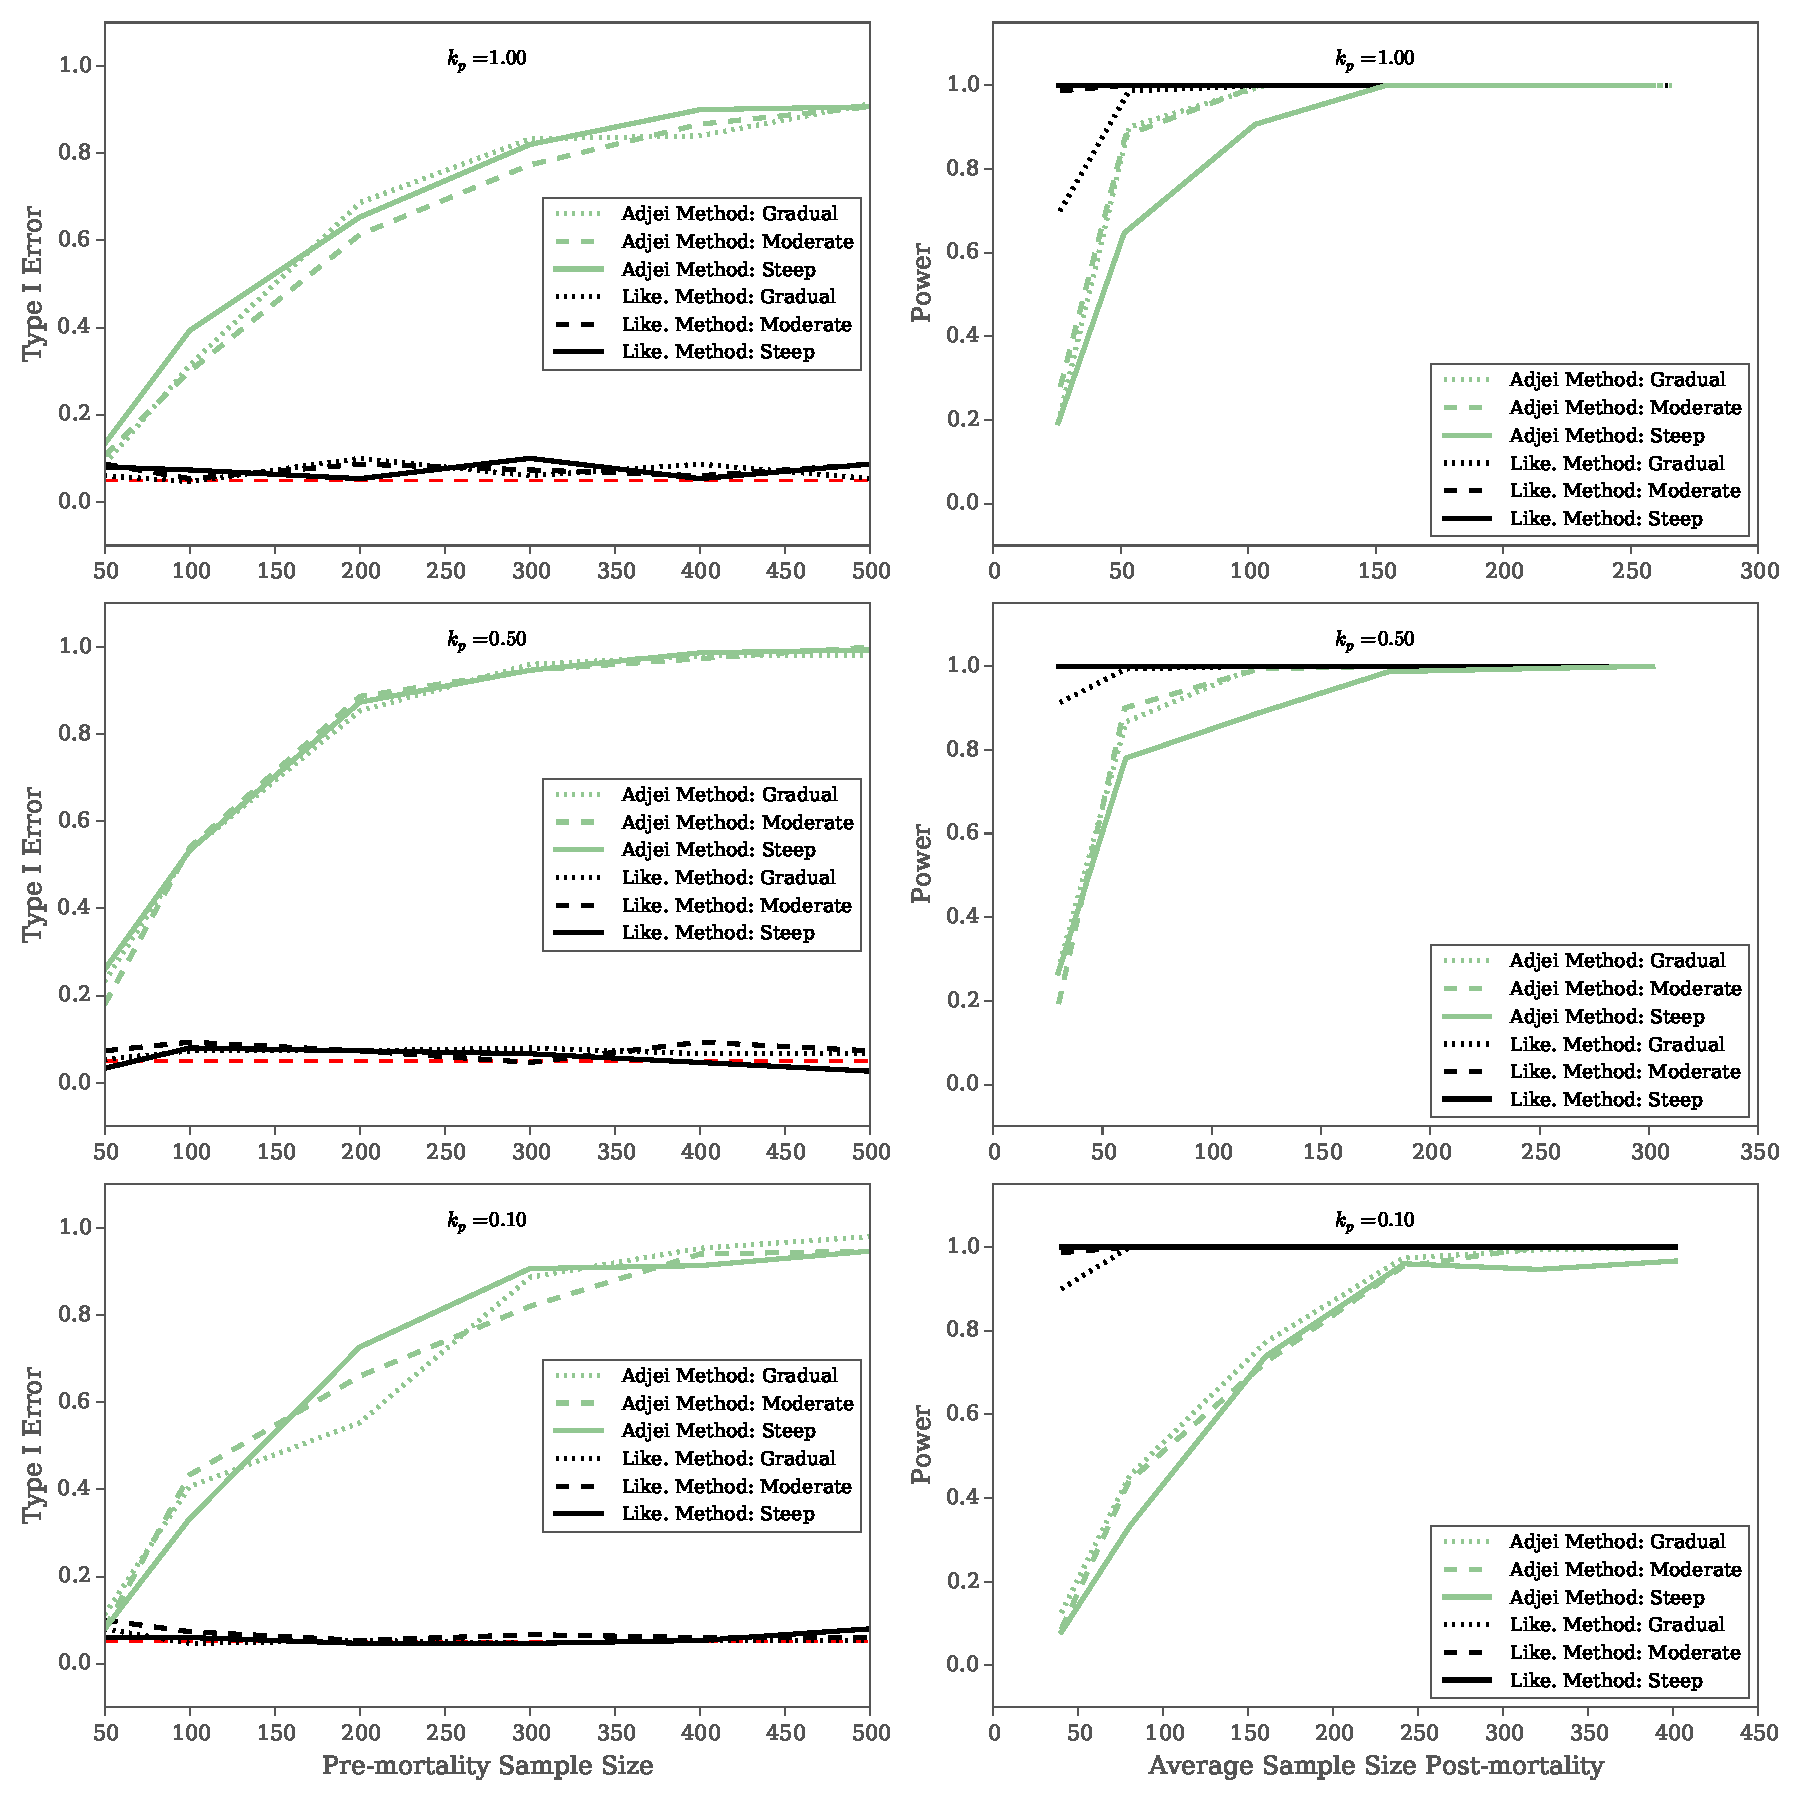
\includegraphics[width=\textwidth]{/Users/mqwilber/Repos/parasite_mortality/results/typeIpower_figure_for_mu50}

    \caption{The type I error rate and the power of the Likelihood Method (solid line) and the Adjei Method (dashed lines) when $\mu_p = 50$ for various shapes of the host survival function and levels of aggregation $k_p$.  The first column gives the type I error rate of each method for falsely detecting PIHM when none is present.  The red line gives the the pre-set type I error rate of $\alpha = 0.05$.  The second column gives the power of a given method to detect PIHM when it is actually occurring. }
    \label{fig:typeI50}

\end{figure}

\begin{figure}

    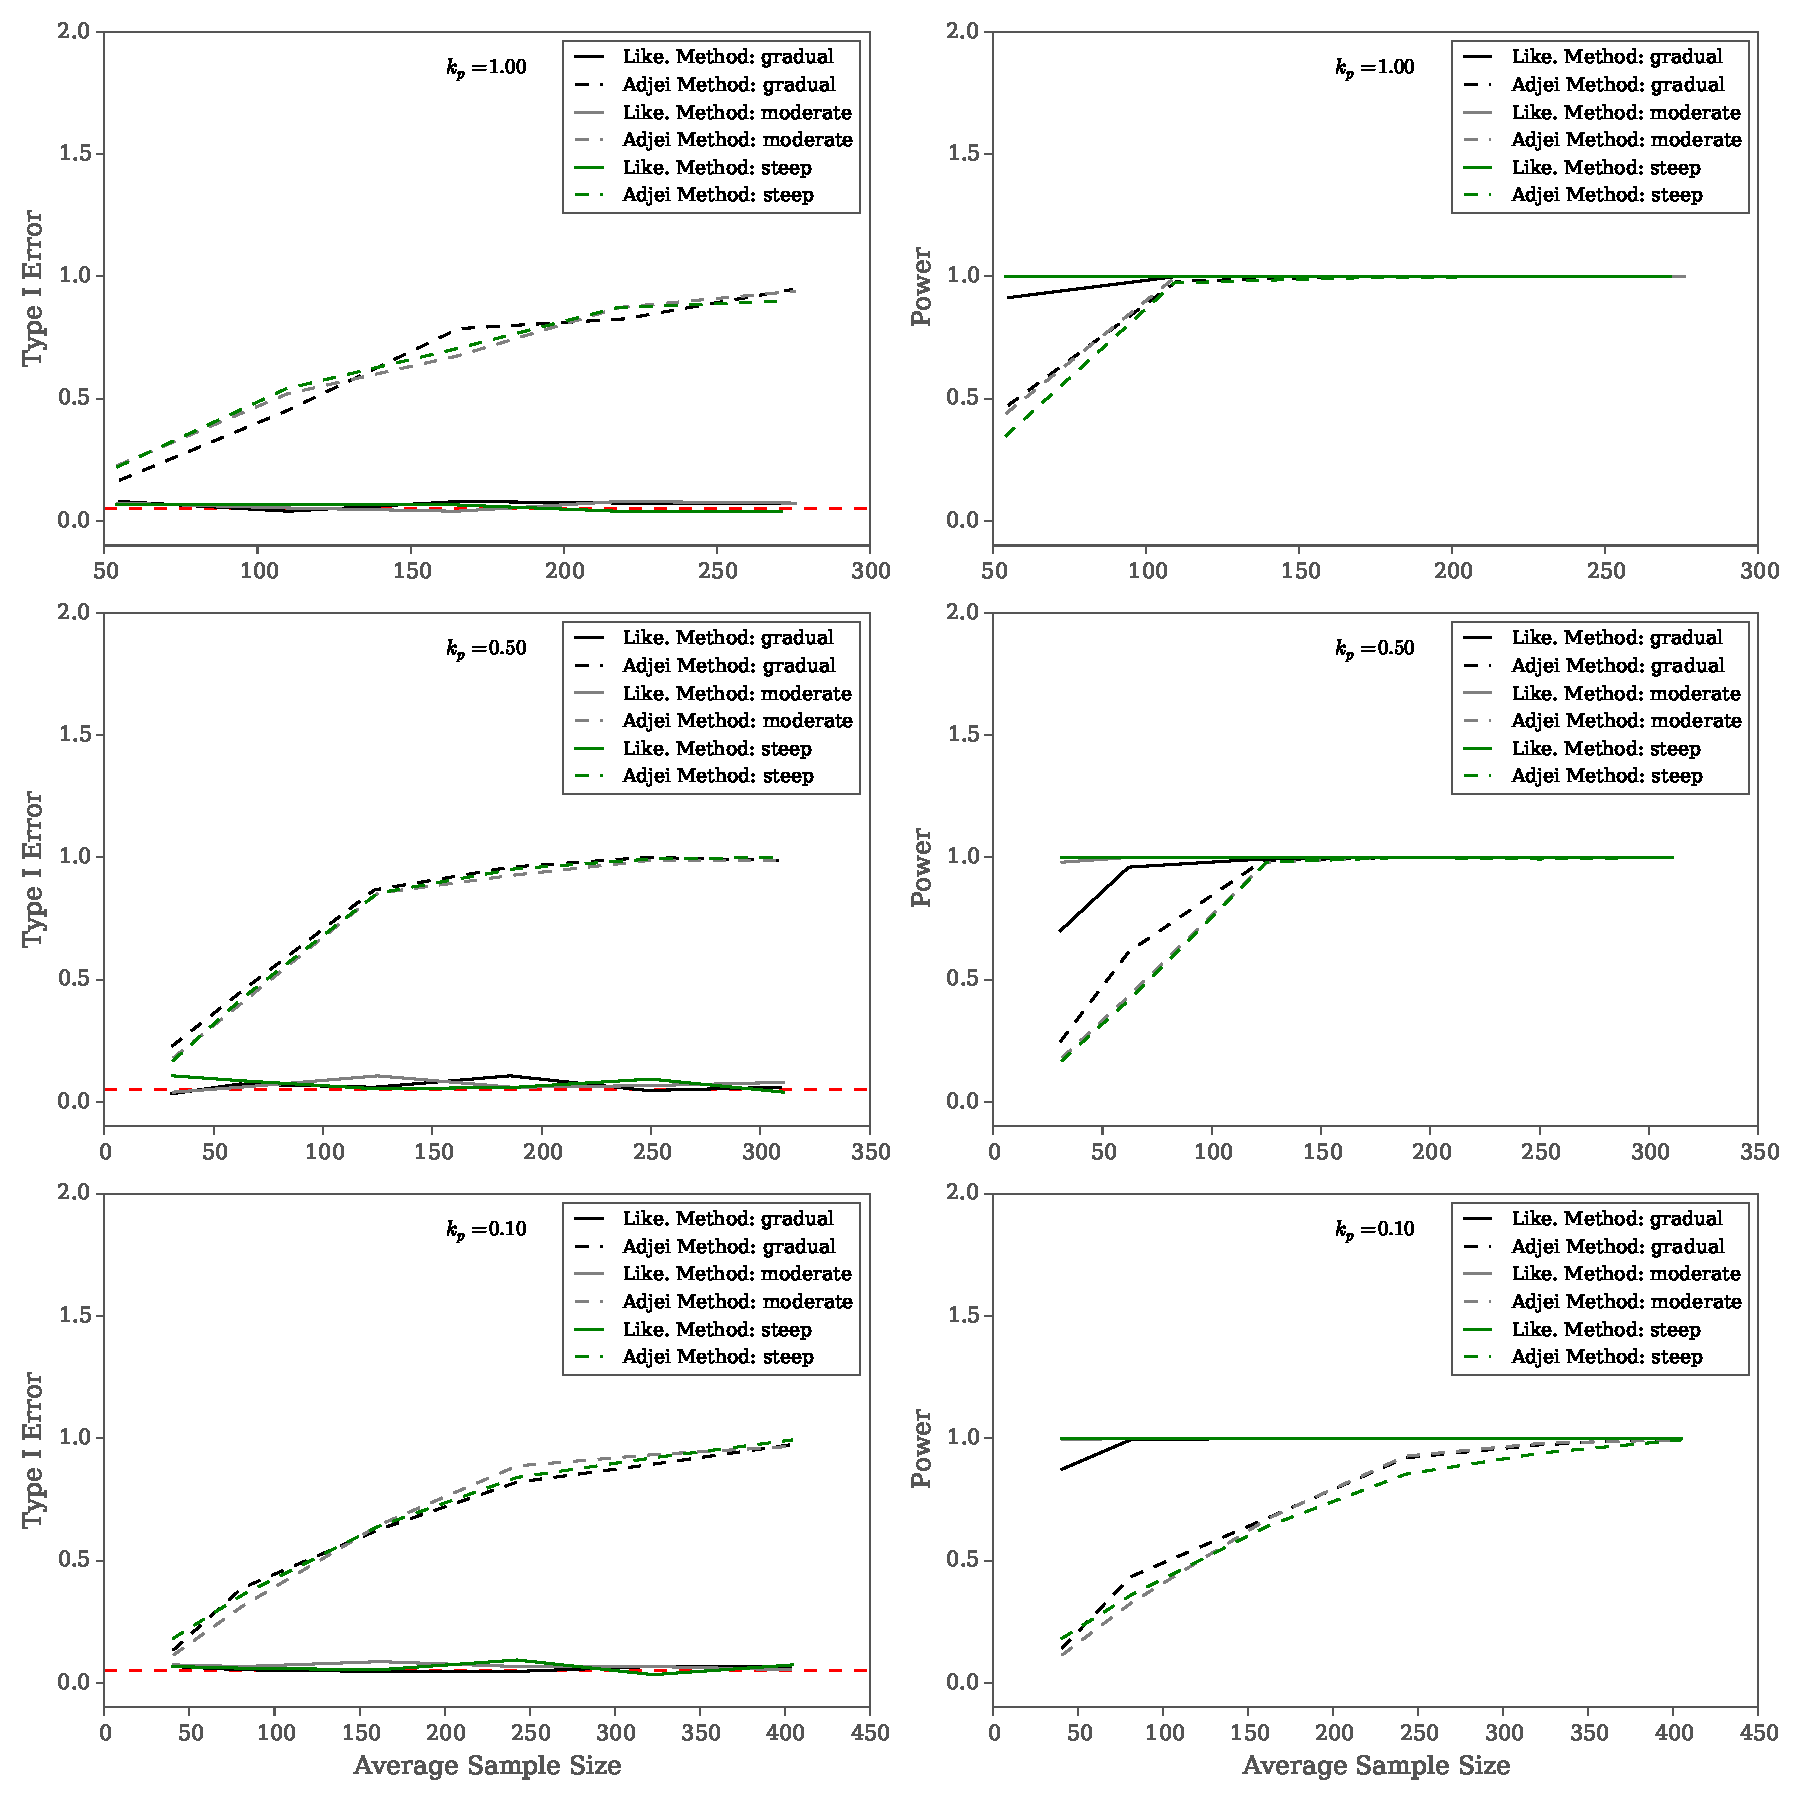
\includegraphics[width=\textwidth]{/Users/mqwilber/Repos/parasite_mortality/results/typeIpower_figure_for_mu100}

    \caption{The type I error rate and the power of the Likelihood Method (solid line) and the Adjei Method (dashed lines) when $\mu_p = 100$ for various shapes of the host survival function and levels of aggregation $k_p$.  The first column gives the type I error rate of each method for falsely detecting PIHM when none is present.  The red line gives the the pre-set type I error rate of $\alpha = 0.05$.  The second column gives the power of a given method to detect PIHM when it is actually occurring. }
    \label{fig:typeI100}

\end{figure}

\begin{figure}

    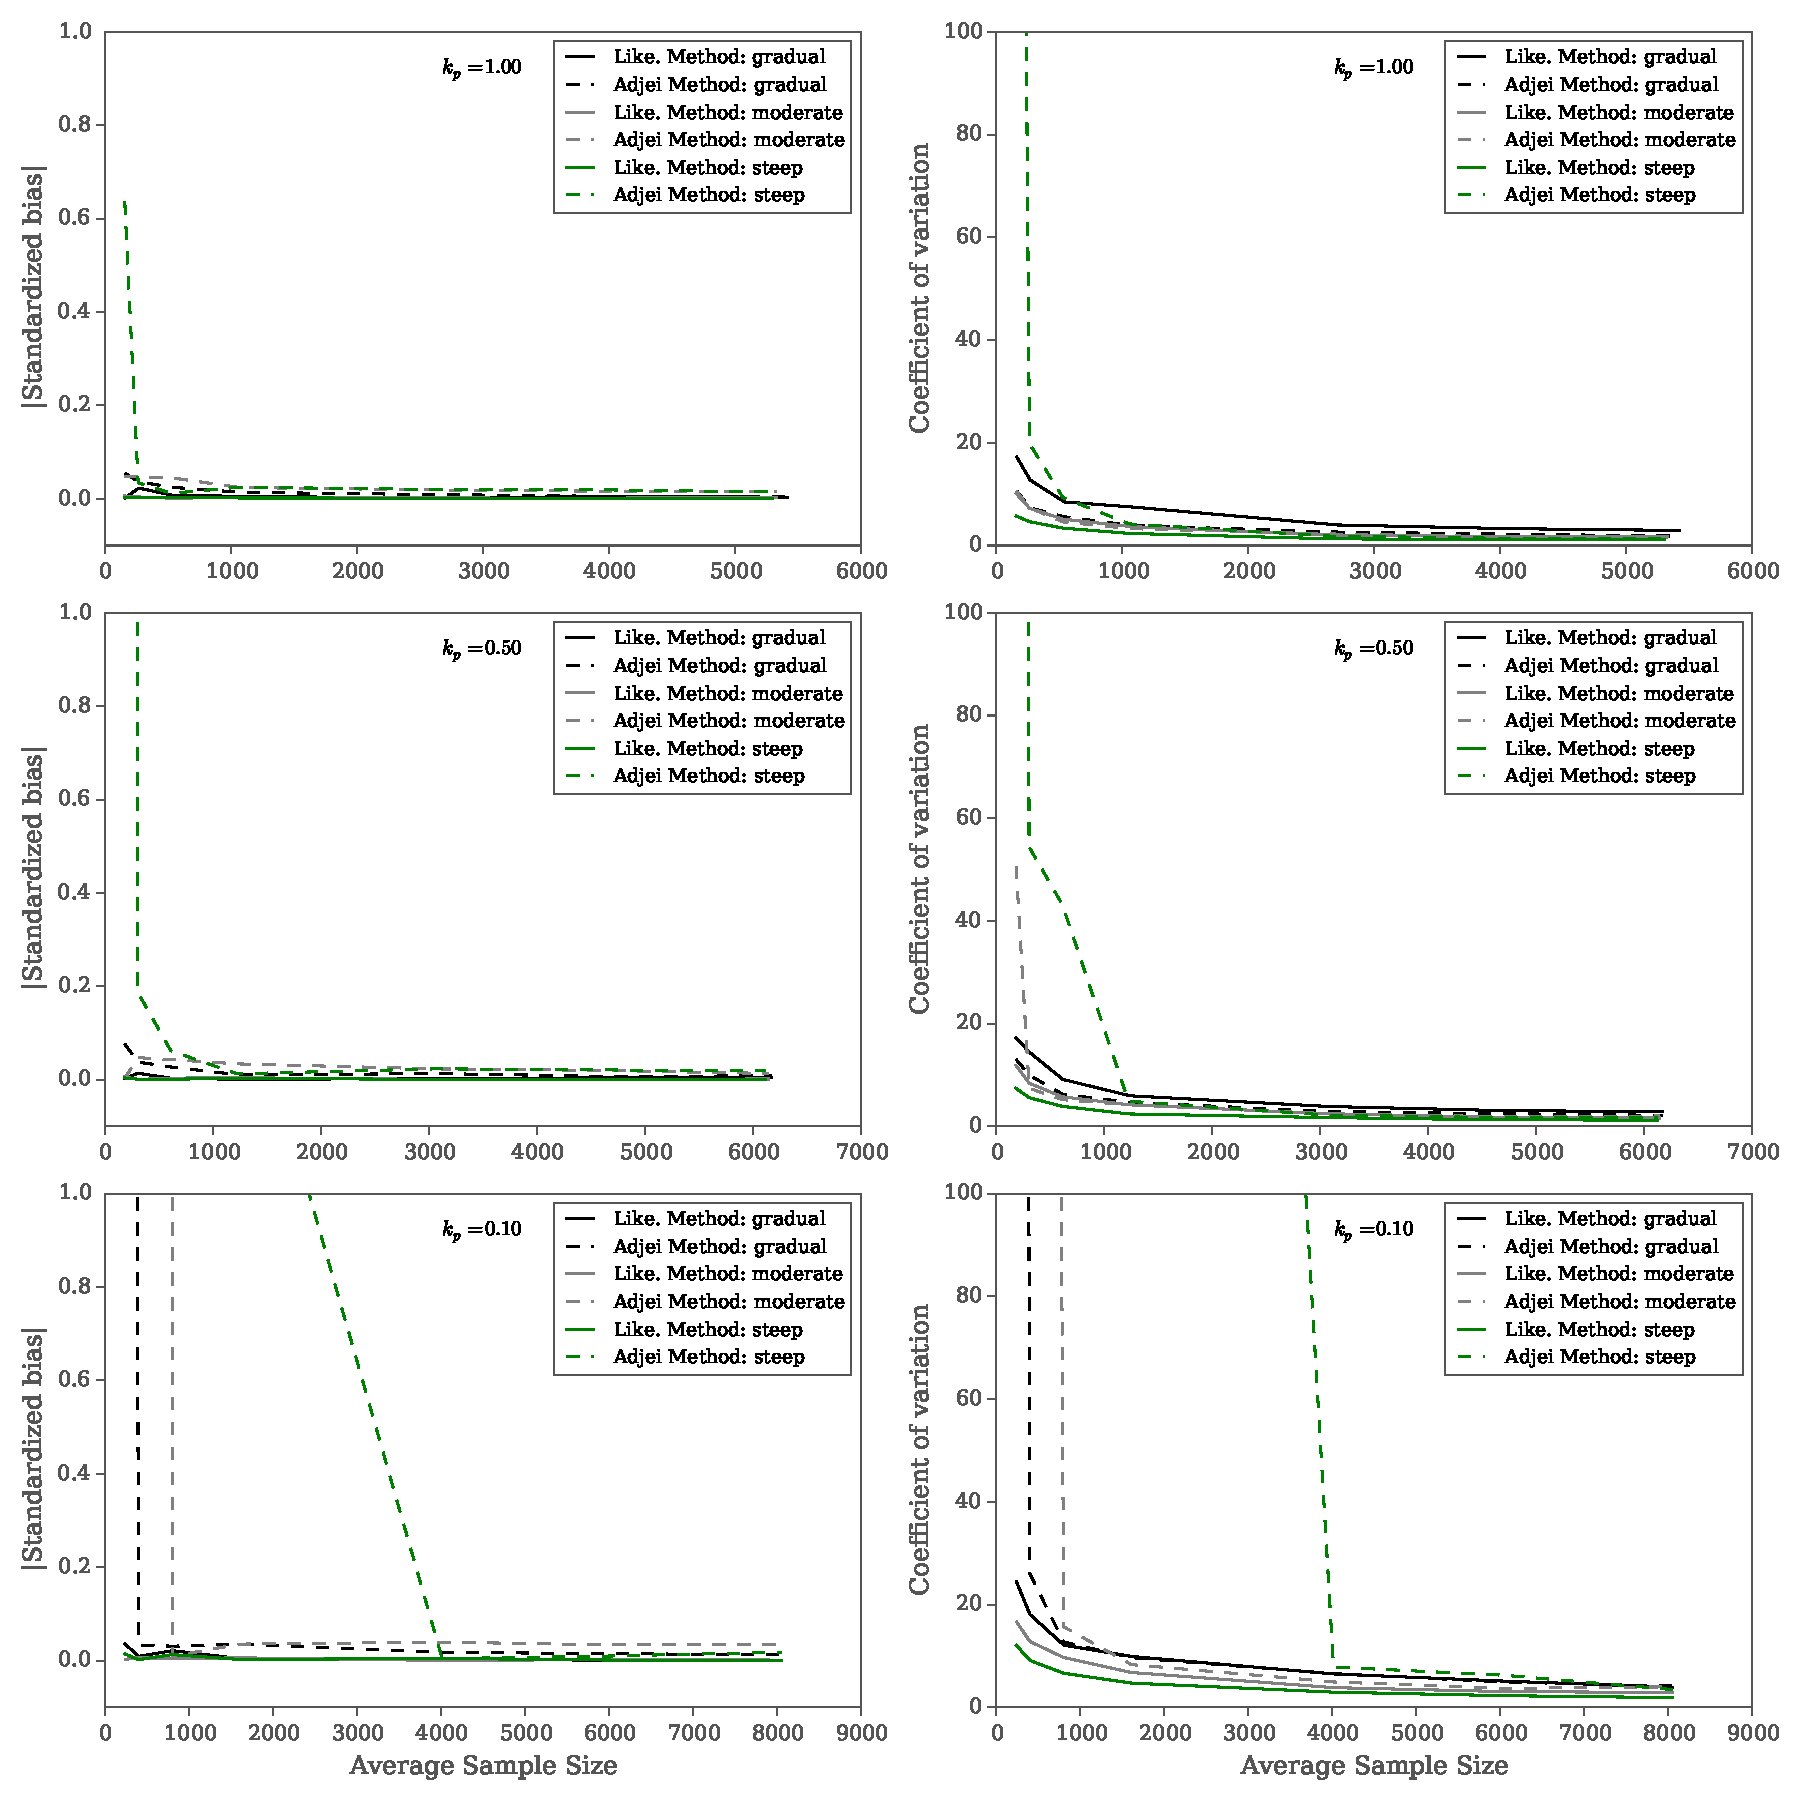
\includegraphics[width=\textwidth]{/Users/mqwilber/Repos/parasite_mortality/results/bais_prec_figure_for_ld50_mu10}

    \caption{The bias and the precision of the Likelihood Method (solid line) and the Adjei Method (dashed lines) when $\mu_p = 10$ for various shapes of the host survival function and levels of aggregation $k_p$ when estimating $LD_{50}$.  The first column gives the bias of each method's $LD_{50}$ estimate over 150 simulations. The second column gives the precision of each method's $LD_{50}$ estimate over 150 simulations.}

    \label{fig:biasld50_10}

\end{figure}

\begin{figure}

    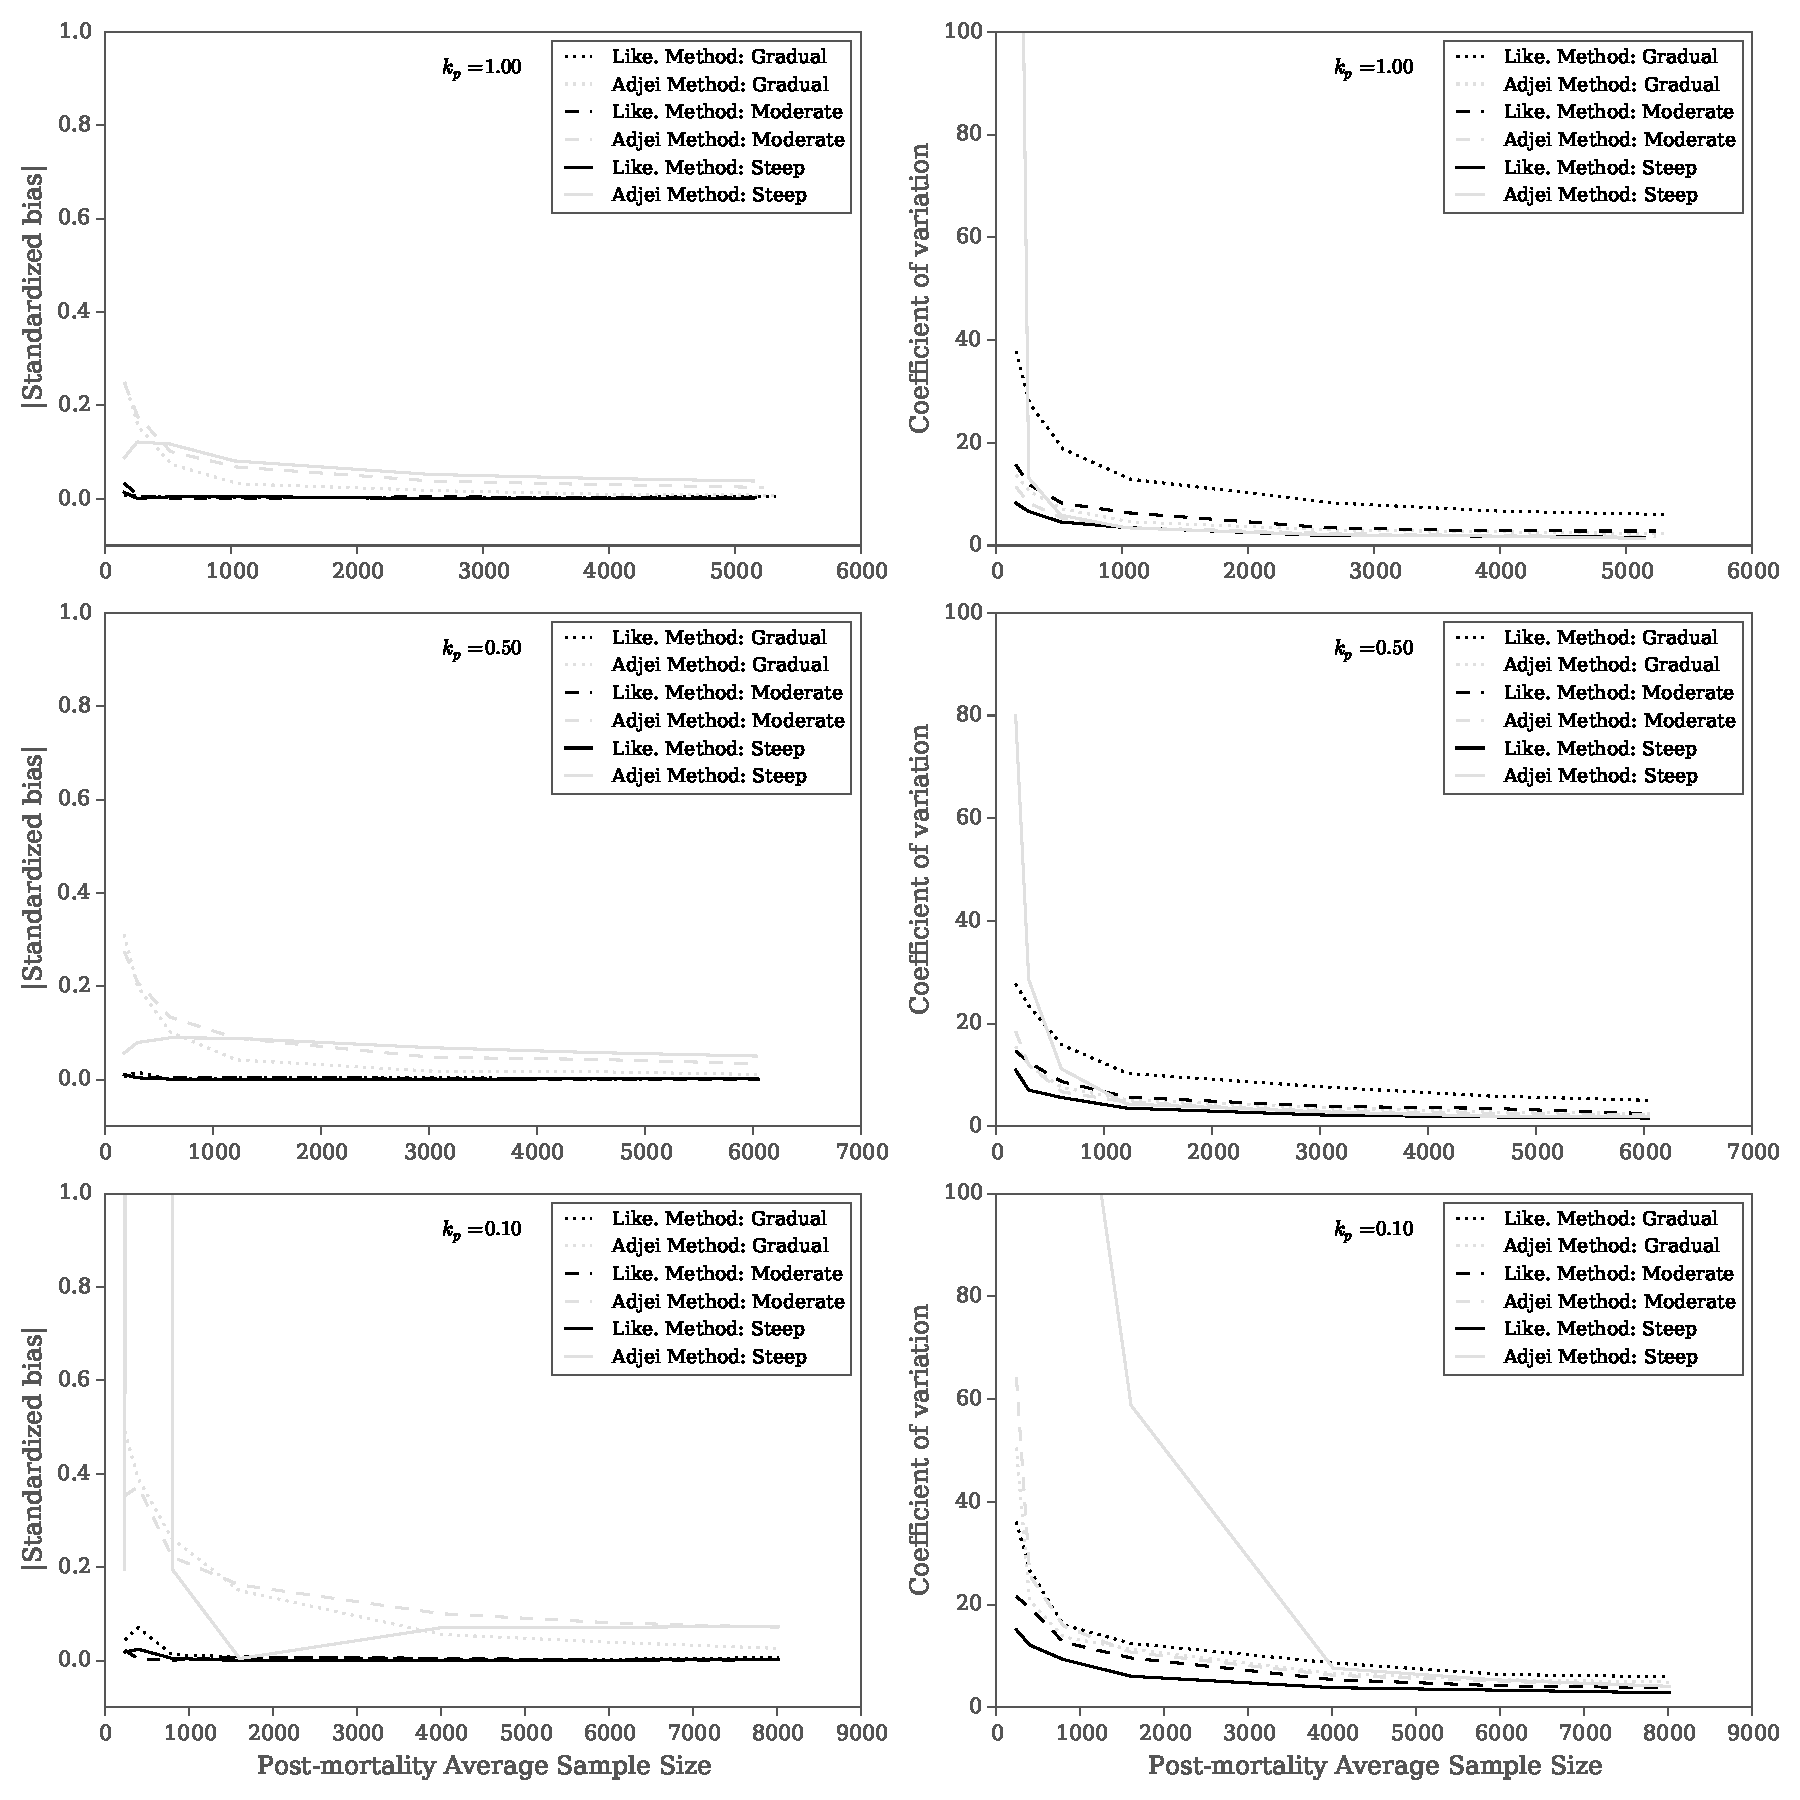
\includegraphics[width=\textwidth]{/Users/mqwilber/Repos/parasite_mortality/results/bais_prec_figure_for_ld50_mu50}

    \caption{The bias and the precision of the Likelihood Method (solid line) and the Adjei Method (dashed lines) when $\mu_p = 50$ for various shapes of the host survival function and levels of aggregation $k_p$ when estimating $LD_{50}$.  The first column gives the bias of each method's $LD_{50}$ estimate over 150 simulations. The second column gives the precision of each method's $LD_{50}$ estimate over 150 simulations.}

    \label{fig:biasld50_50}

\end{figure}

\begin{figure}

    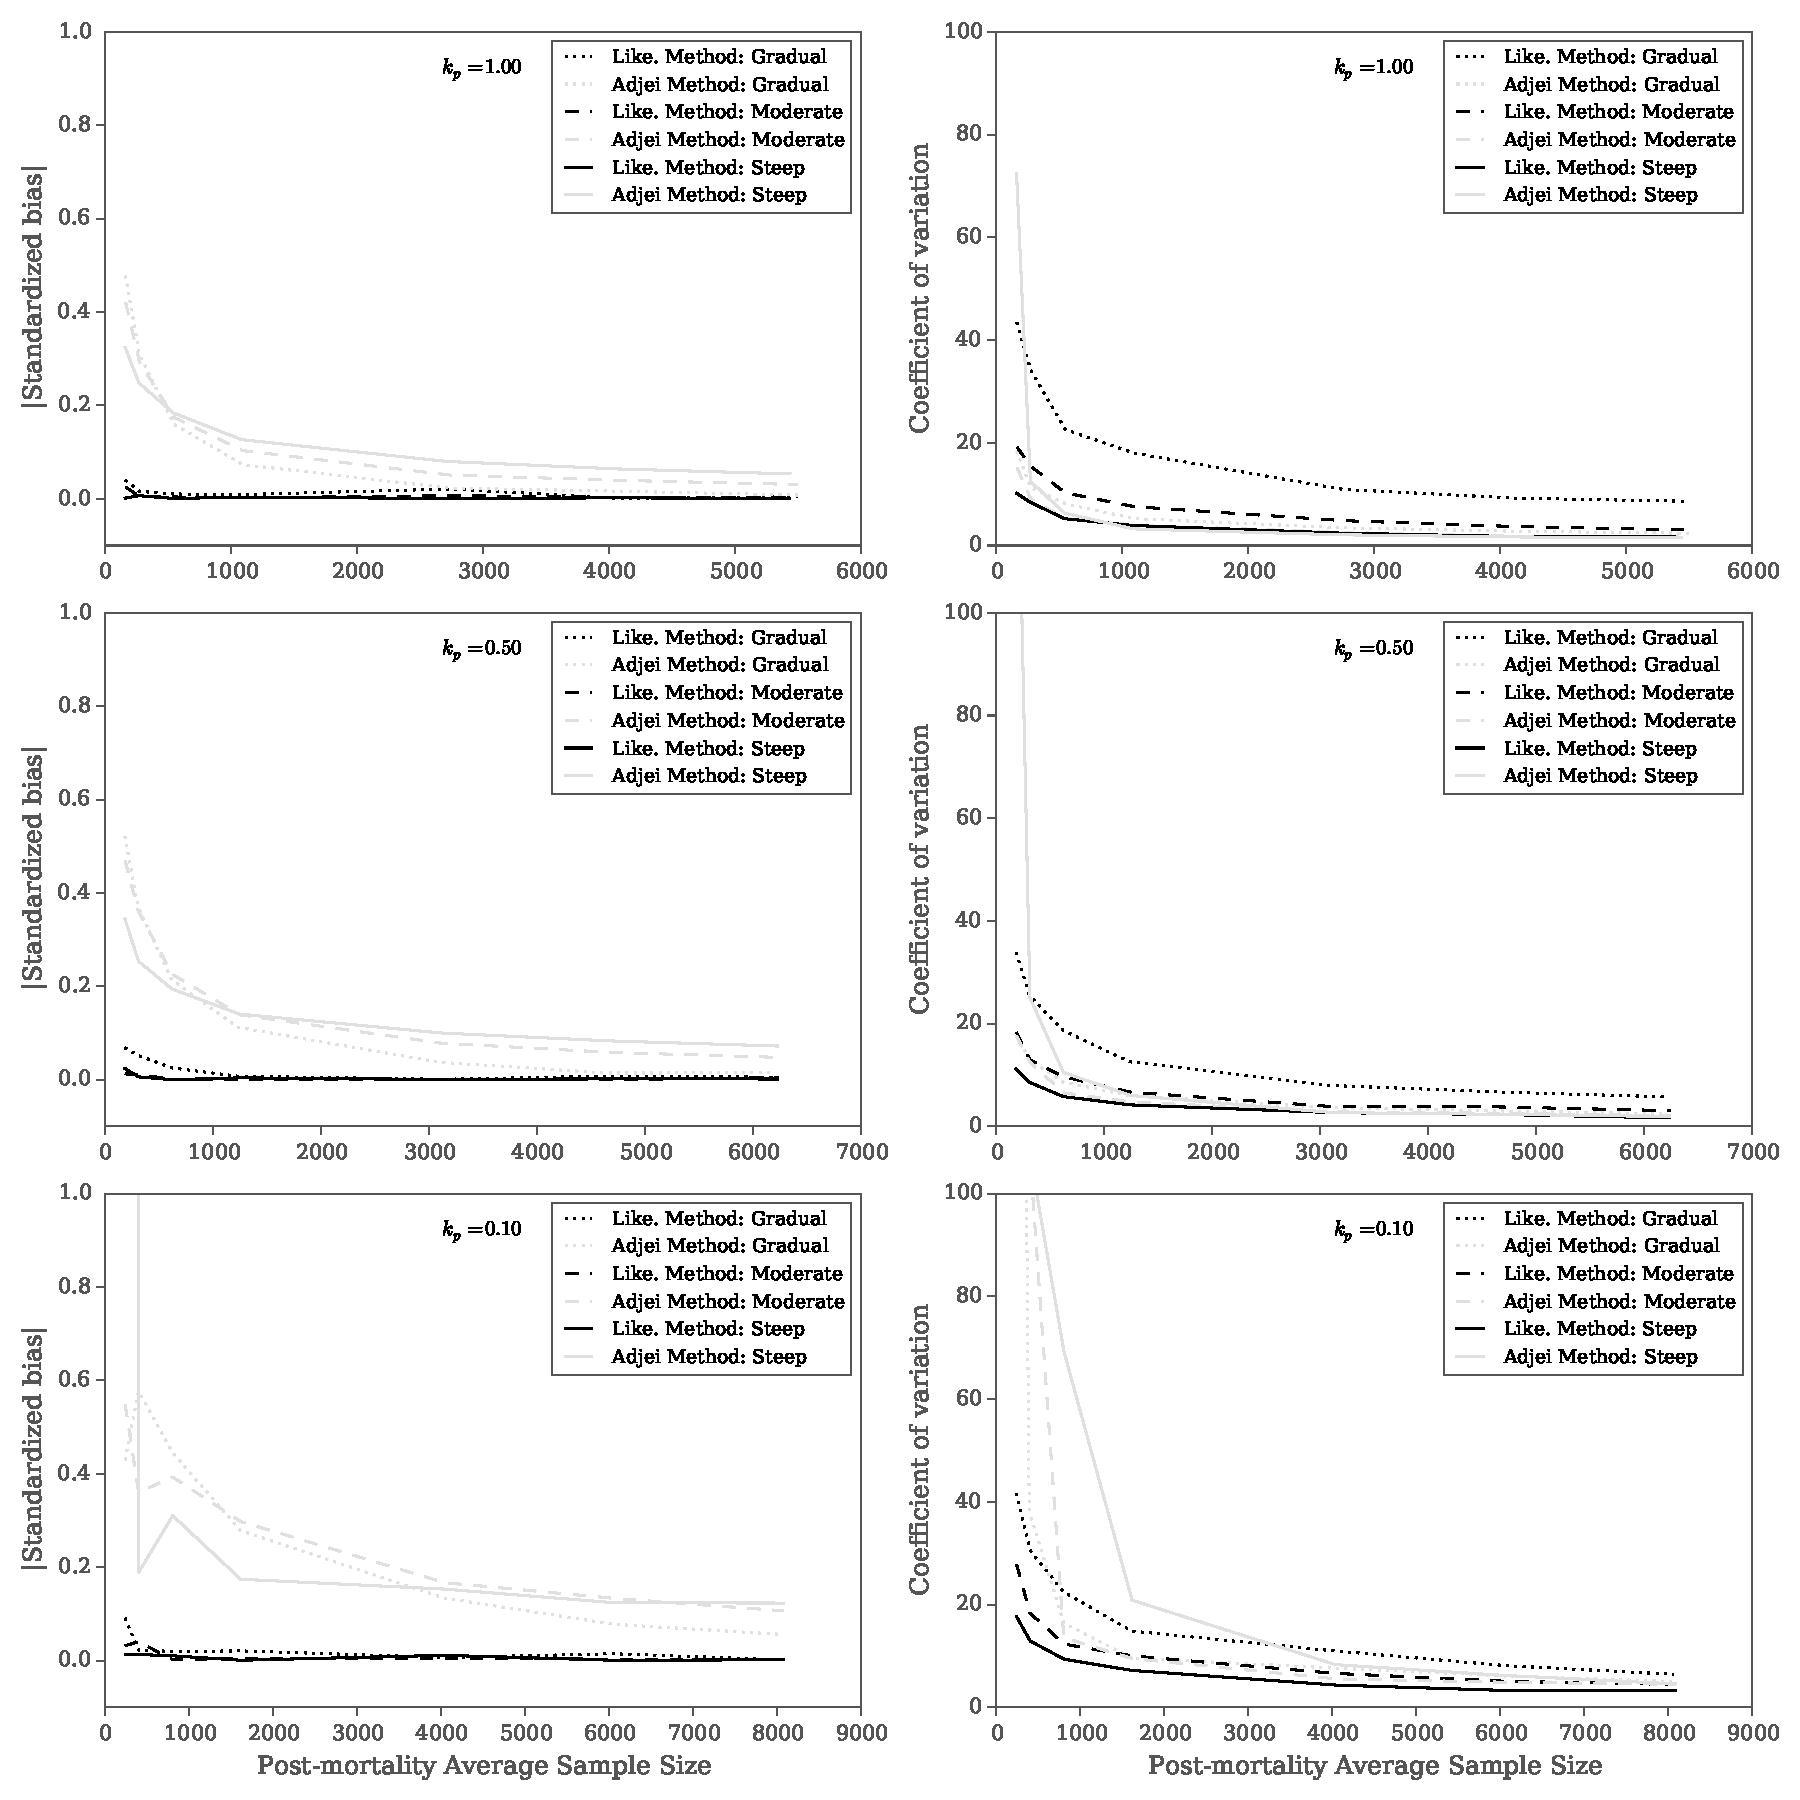
\includegraphics[width=\textwidth]{/Users/mqwilber/Repos/parasite_mortality/results/bais_prec_figure_for_ld50_mu100}

    \caption{The bias and the precision of the Likelihood Method (solid line) and the Adjei Method (dashed lines) when $\mu_p = 100$ for various shapes of the host survival function and levels of aggregation $k_p$ when estimating $LD_{50}$.  The first column gives the bias of each method's $LD_{50}$ estimate over 150 simulations. The second column gives the precision of each method's $LD_{50}$ estimate over 150 simulations.}

    \label{fig:biasld50_100}

\end{figure}

\begin{figure}

    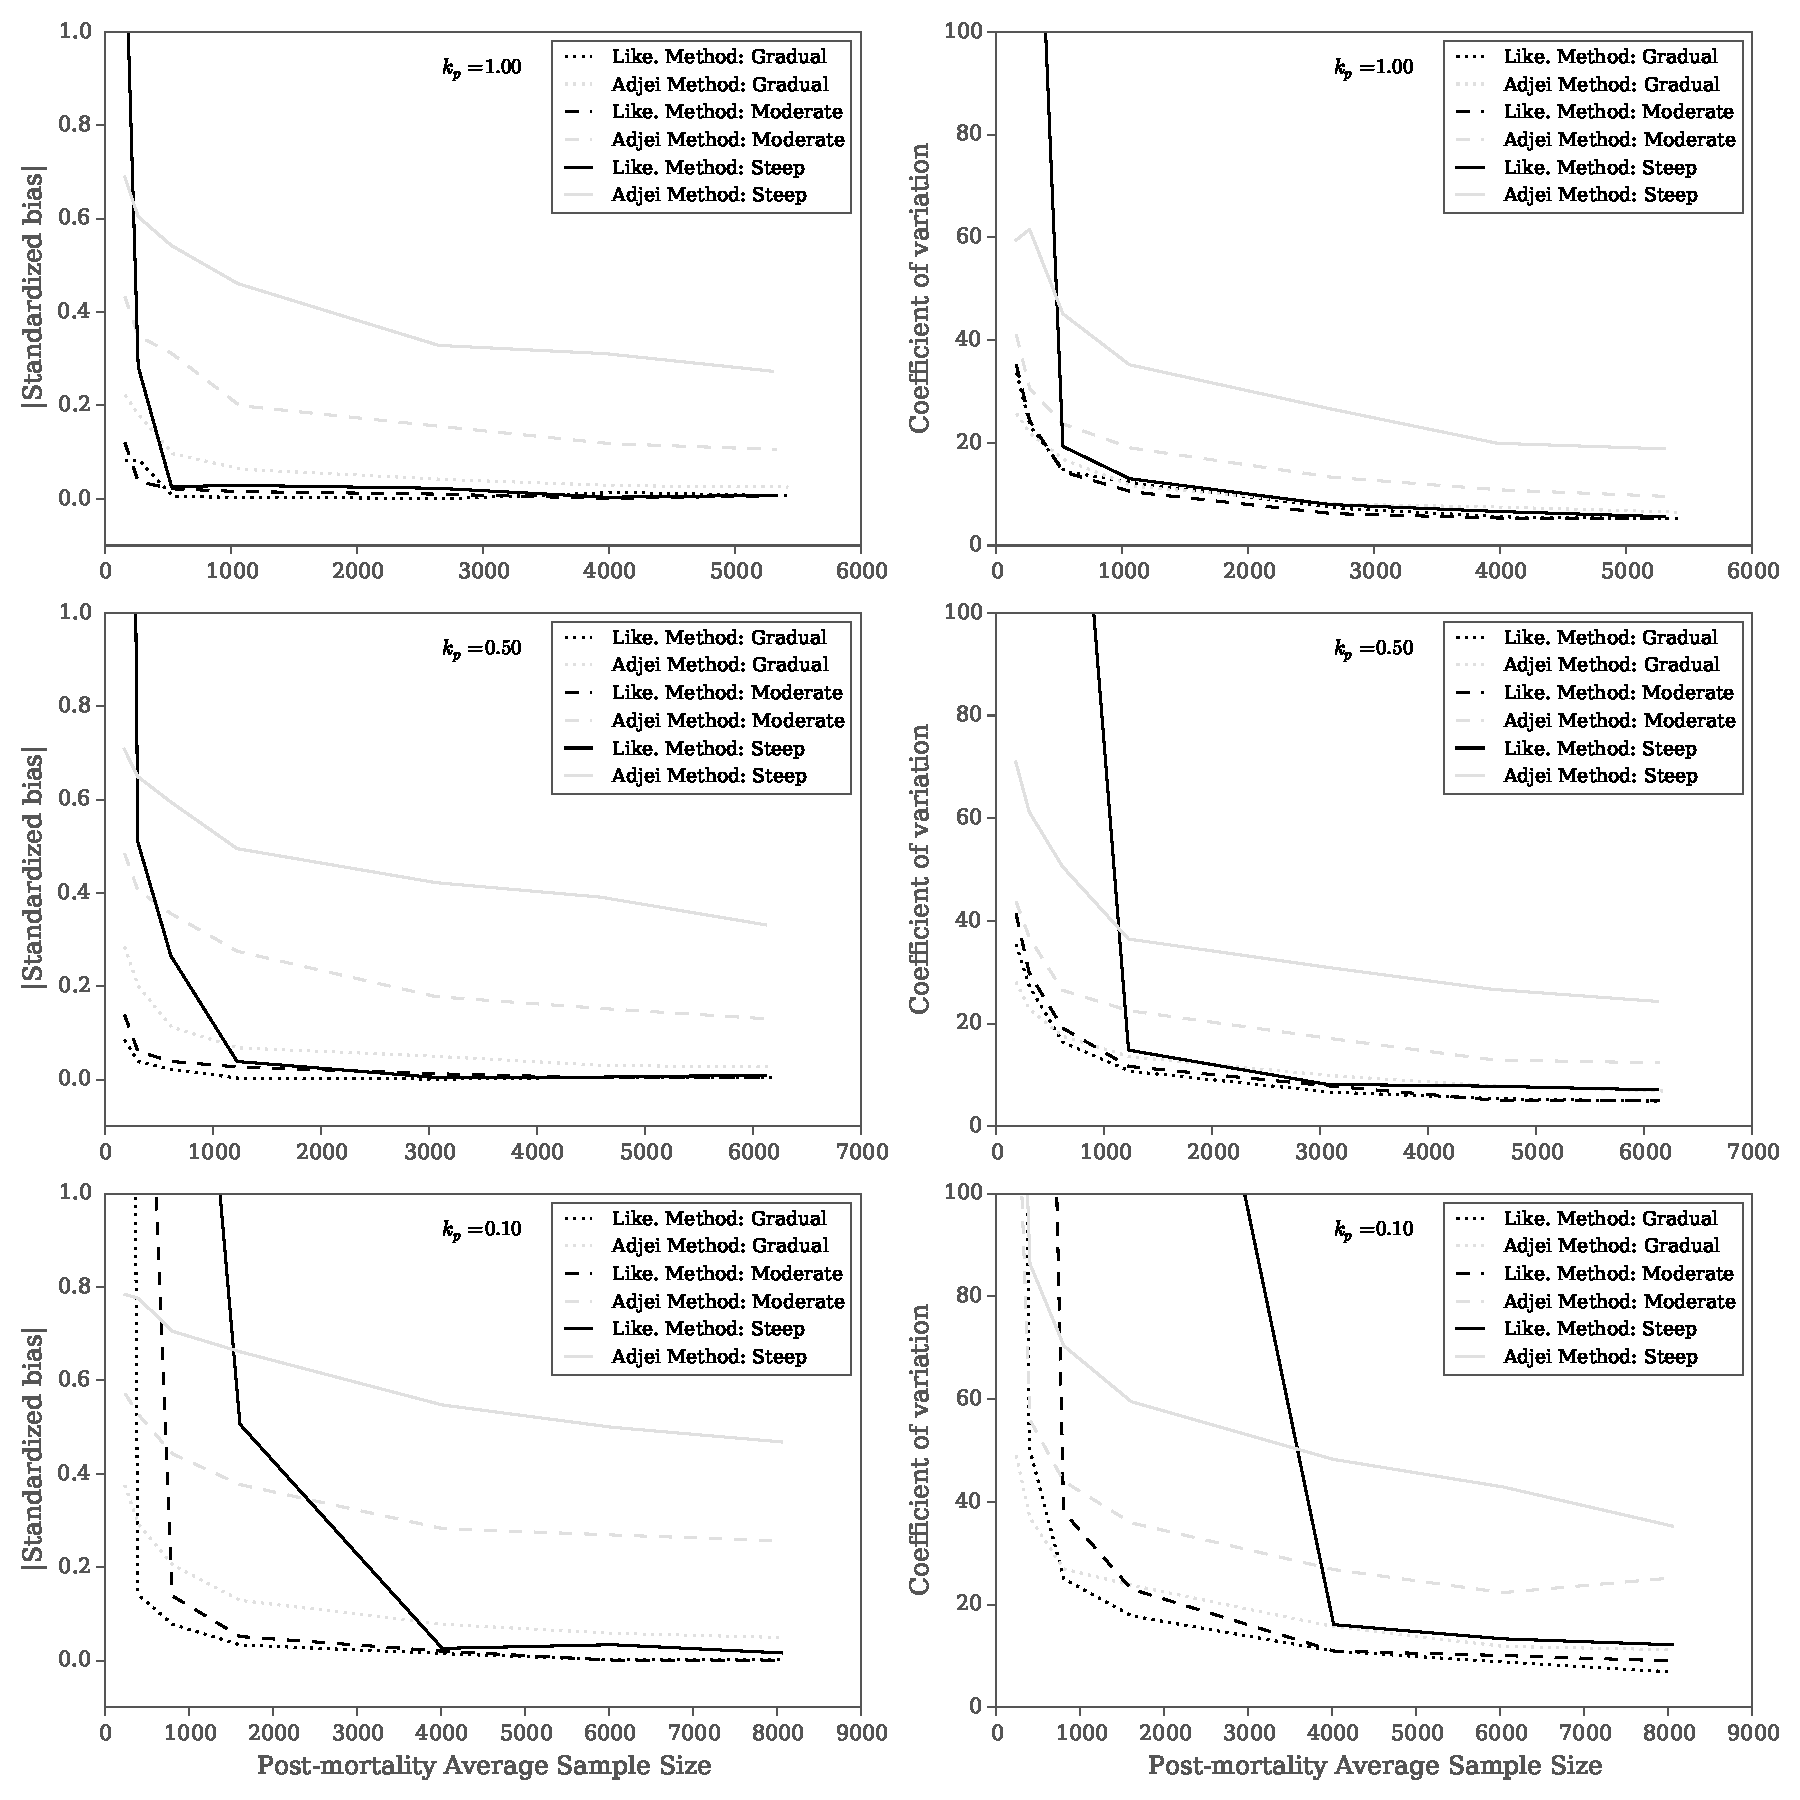
\includegraphics[width=\textwidth]{/Users/mqwilber/Repos/parasite_mortality/results/bais_prec_figure_for_a_mu10}

    \caption{The bias and the precision of the Likelihood Method (solid line) and the Adjei Method (dashed lines) when $\mu_p = 10$ for various shapes of the host survival function and levels of aggregation $k_p$ when estimating the $a$ parameter of the host survival function.  The first column gives the bias of each method's $a$ estimate over 150 simulations. The second column gives the precision of each method's $a$ estimate over 150 simulations.}

    \label{fig:biasa_10}

\end{figure}

\begin{figure}

    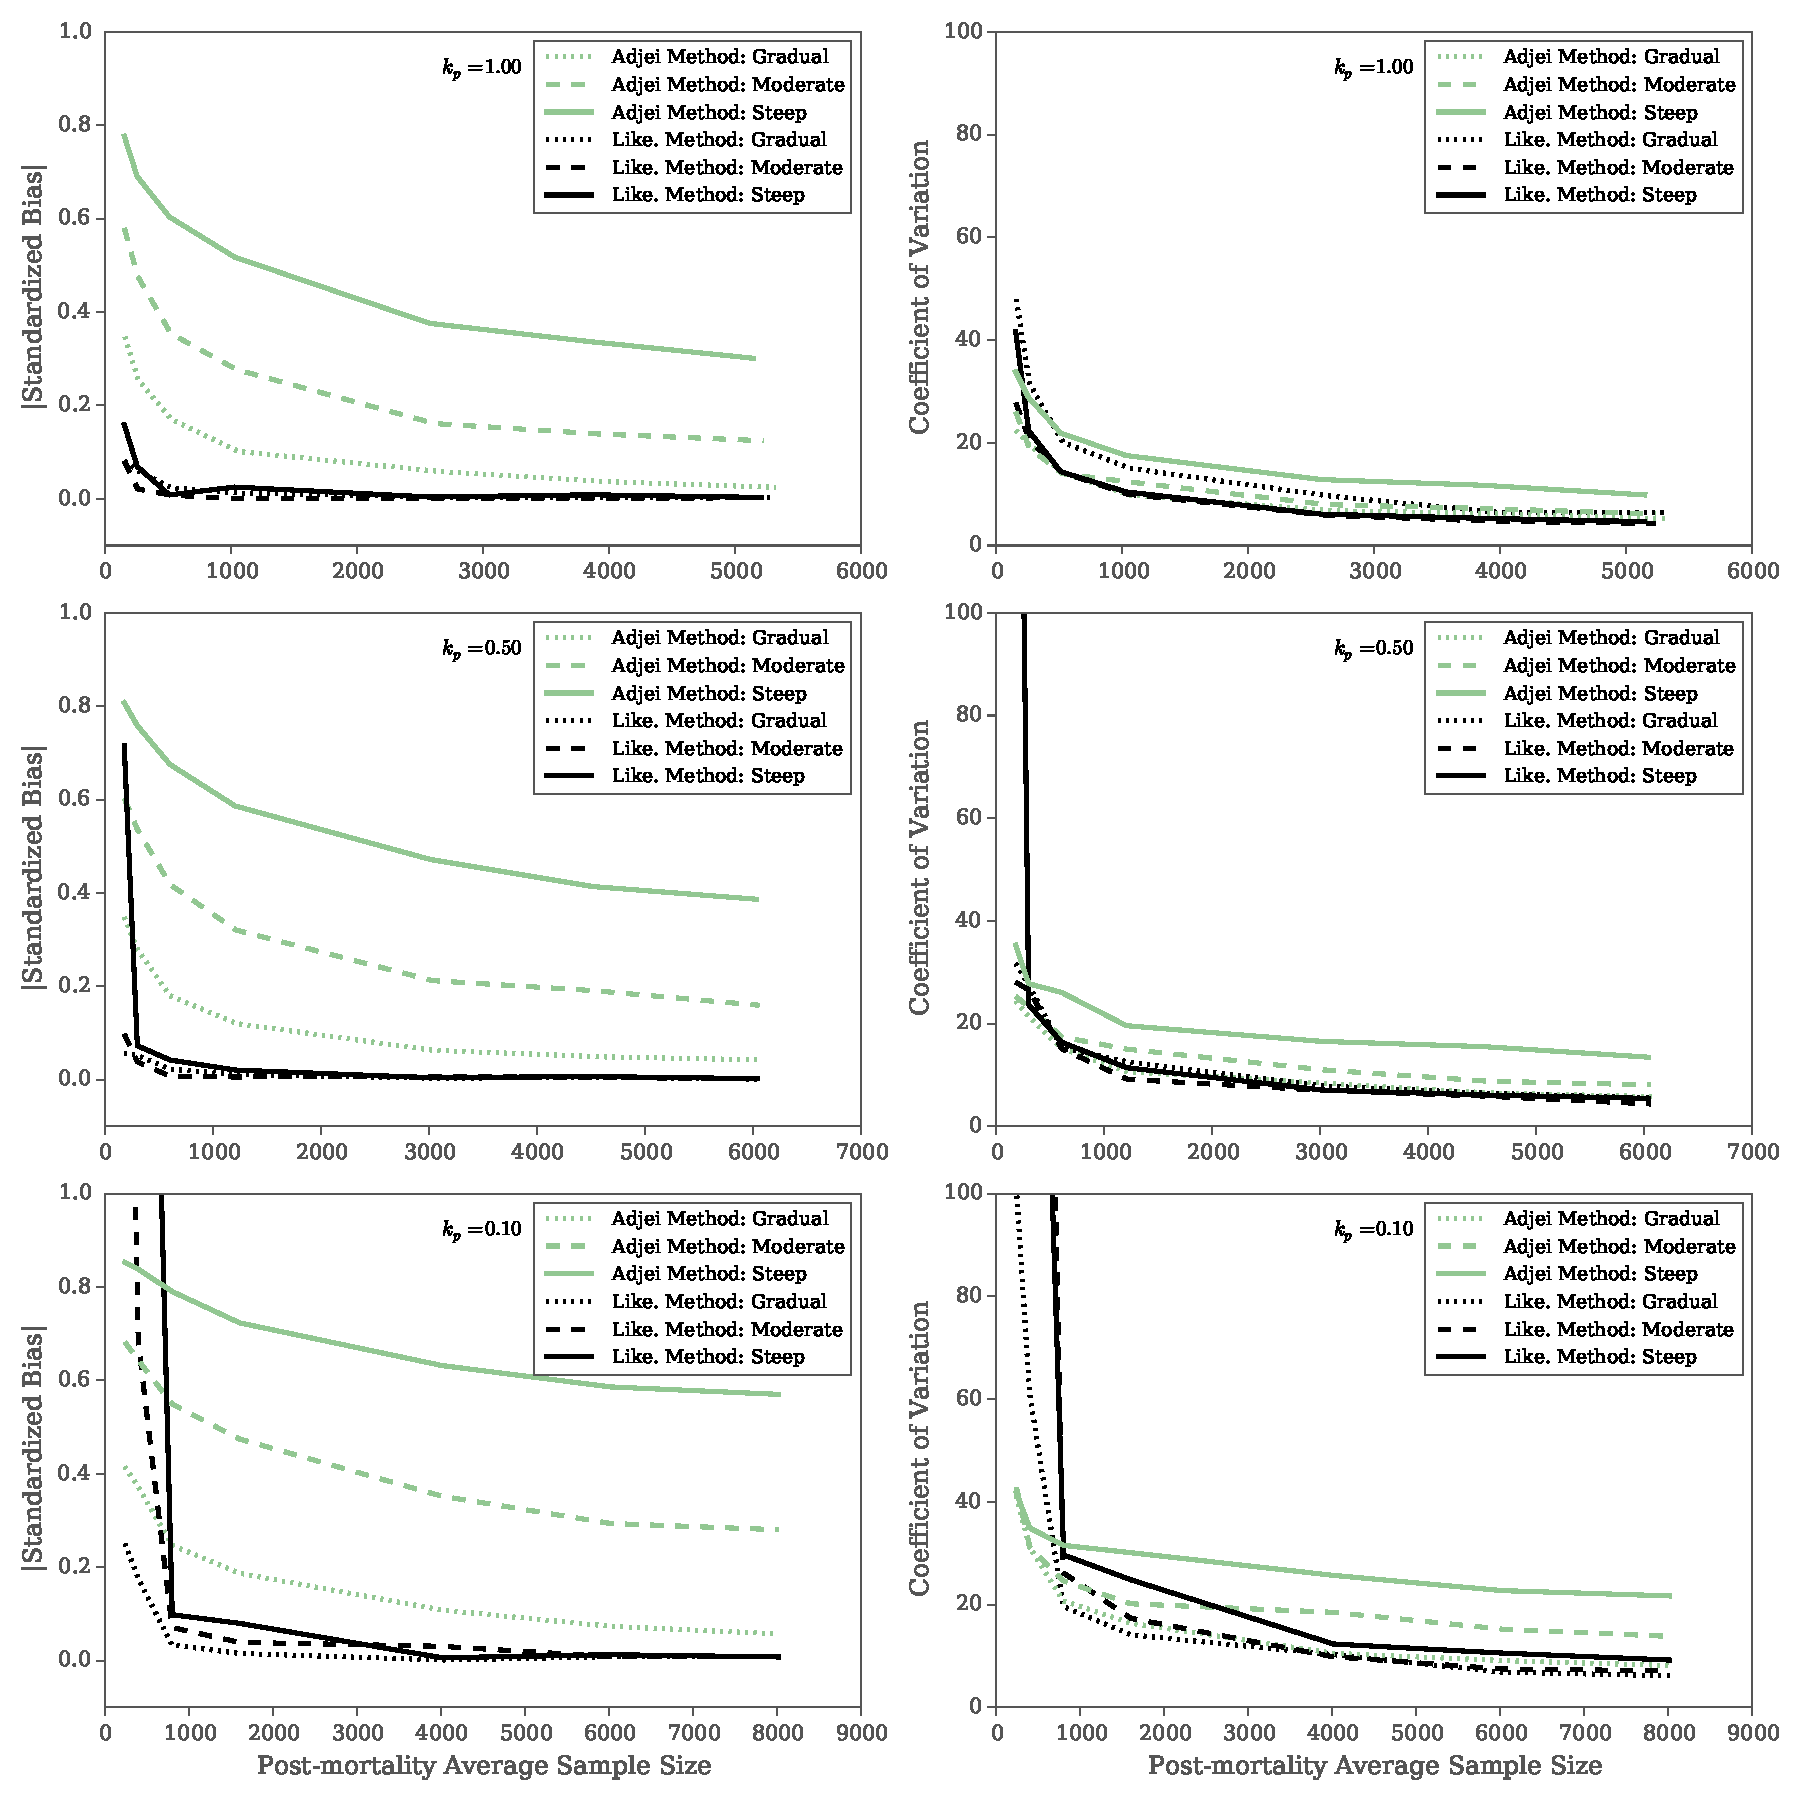
\includegraphics[width=\textwidth]{/Users/mqwilber/Repos/parasite_mortality/results/bais_prec_figure_for_a_mu50}

    \caption{The bias and the precision of the Likelihood Method (solid line) and the Adjei Method (dashed lines) when $\mu_p = 50$ for various shapes of the host survival function and levels of aggregation $k_p$ when estimating the $a$ parameter of the host survival function.  The first column gives the bias of each method's $a$ estimate over 150 simulations. The second column gives the precision of each method's $a$ estimate over 150 simulations.}

    \label{fig:biasa_50}

\end{figure}

\begin{figure}

    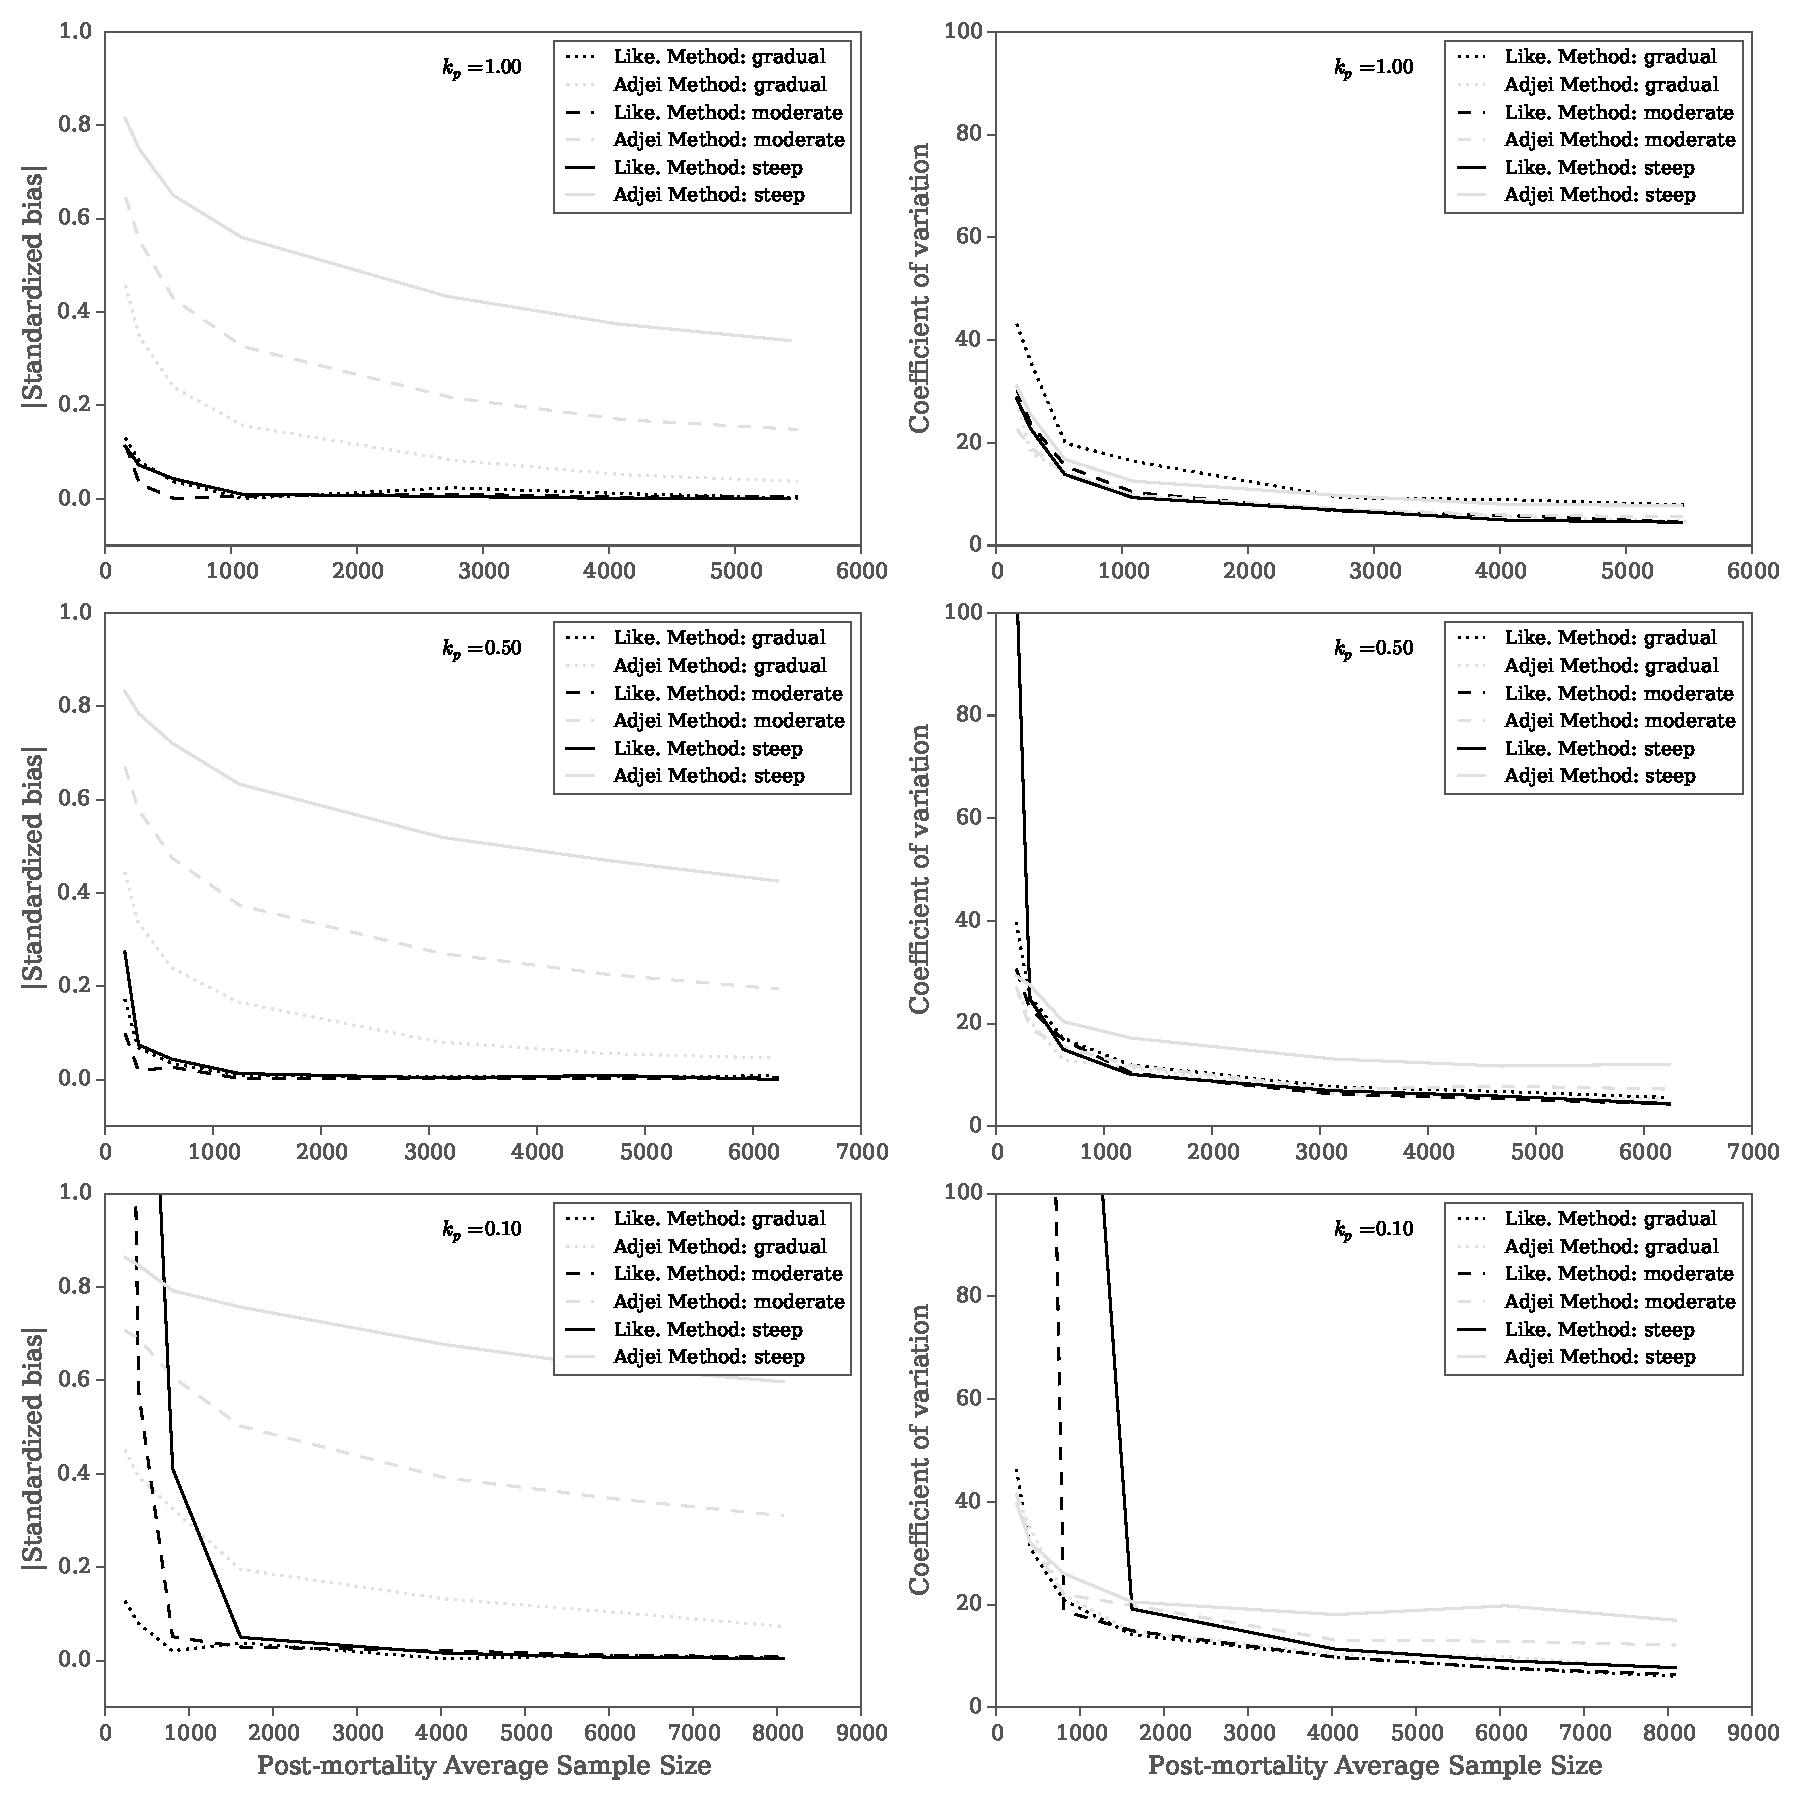
\includegraphics[width=\textwidth]{/Users/mqwilber/Repos/parasite_mortality/results/bais_prec_figure_for_a_mu100}

    \caption{The bias and the precision of the Likelihood Method (solid line) and the Adjei Method (dashed lines) when $\mu_p = 100$ for various shapes of the host survival function and levels of aggregation $k_p$ when estimating the $a$ parameter of the host survival function.  The first column gives the bias of each method's $a$ estimate over 150 simulations. The second column gives the precision of each method's $a$ estimate over 150 simulations.}

    \label{fig:biasa_100}

\end{figure}

\begin{figure}
    \centering
    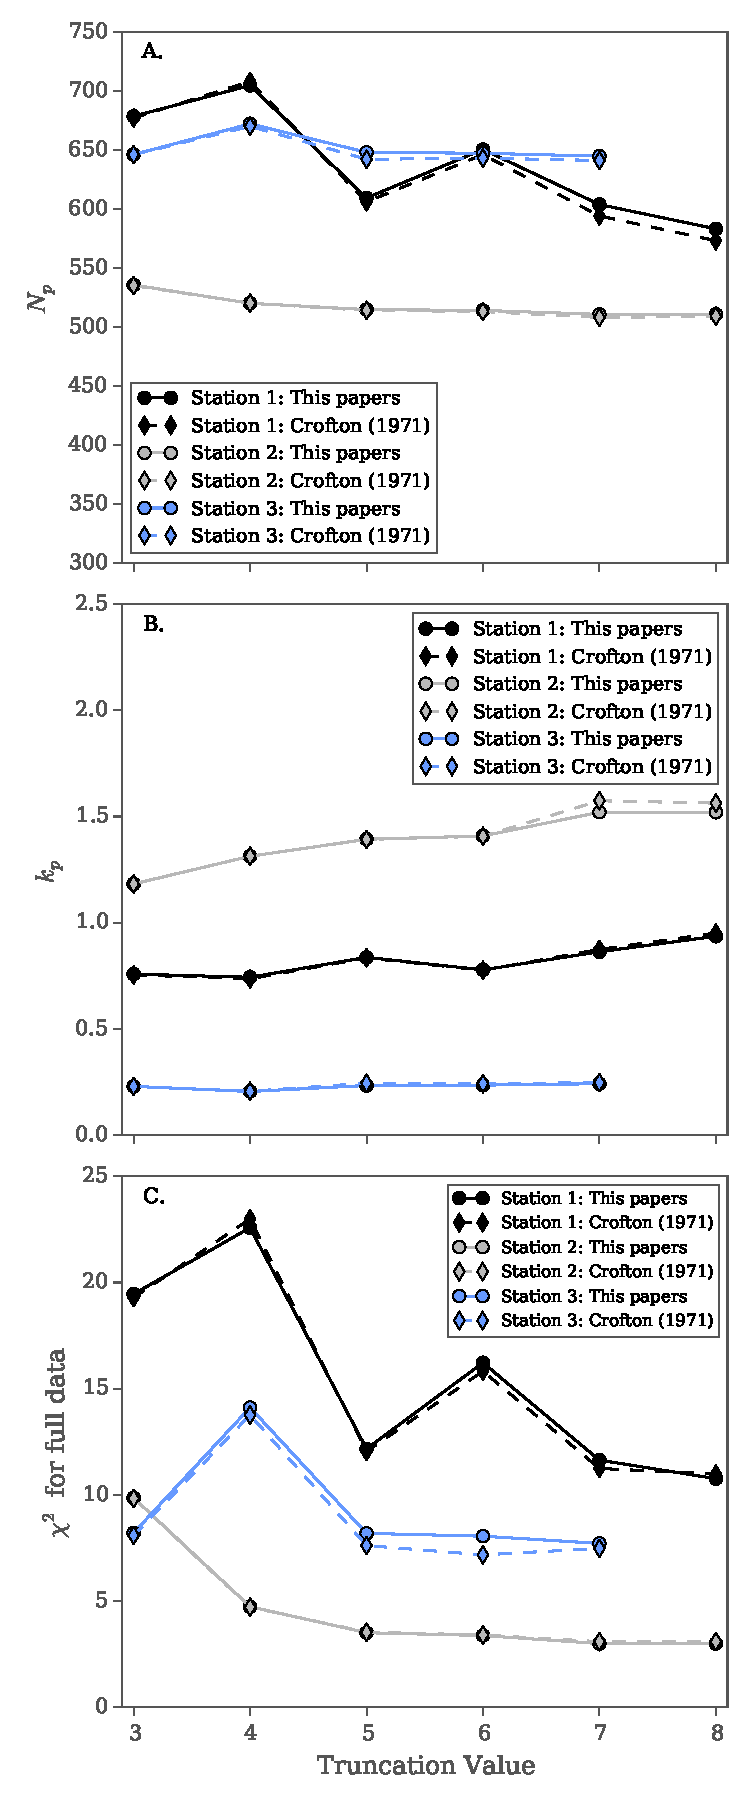
\includegraphics[width=0.5\textwidth]{/Users/mqwilber/Repos/parasite_mortality/results/compare_crofton.pdf}
    \caption{A comparison of this paper's implementation (solid line, circles) of the Crofton Method with the results given in \cite{Crofton1971a} (dashed line, diamonds).  Figure A compares the predicted number of hosts in a population pre-mortality ($N_p$). Figure B compares the predicted parasite aggregation pre-mortality ($k_p$).  Figure C compares the $\chi^2$ statistic for each implementation.  Three of the 6 stations fit by \citeauthor{Crofton1971a} are shown here and all show that our implementation gives very similar results to those given by \citeauthor{Crofton1971a}.}
    \label{fig:crof_test}

\end{figure}


\end{document}

